%###########################PRESENTACION##########################################
%Modo presentación
\documentclass[14pt]{beamer}

%Modo handout
%\documentclass[handout,compress]{beamer}
%\usepackage{pgfpages}
%\pgfpagesuselayout{4 on 1}[border shrink=1mm]

\usepackage{graphicx}
\usepackage{beamerthemeCambridgeUS}
\usepackage{subfig}
\usepackage{tikz}
\usepackage{amsmath}
\setbeamercovered{transparent}
\usepackage{xcolor}
\usepackage{textpos} 

\graphicspath{{G:/My Drive/FIGURAS/}}

\title[Sensores Remotos]{ANÁLISIS GEOESPACIAL}
\author[Edier Aristizábal]{Edier V. Aristizábal G.}
\institute{\emph{evaristizabalg@unal.edu.co}}
\date{(Versión:\today)}


\addtobeamertemplate{headline}{}{%
	\begin{textblock*}{2mm}(.9\textwidth,0cm)
	\hfill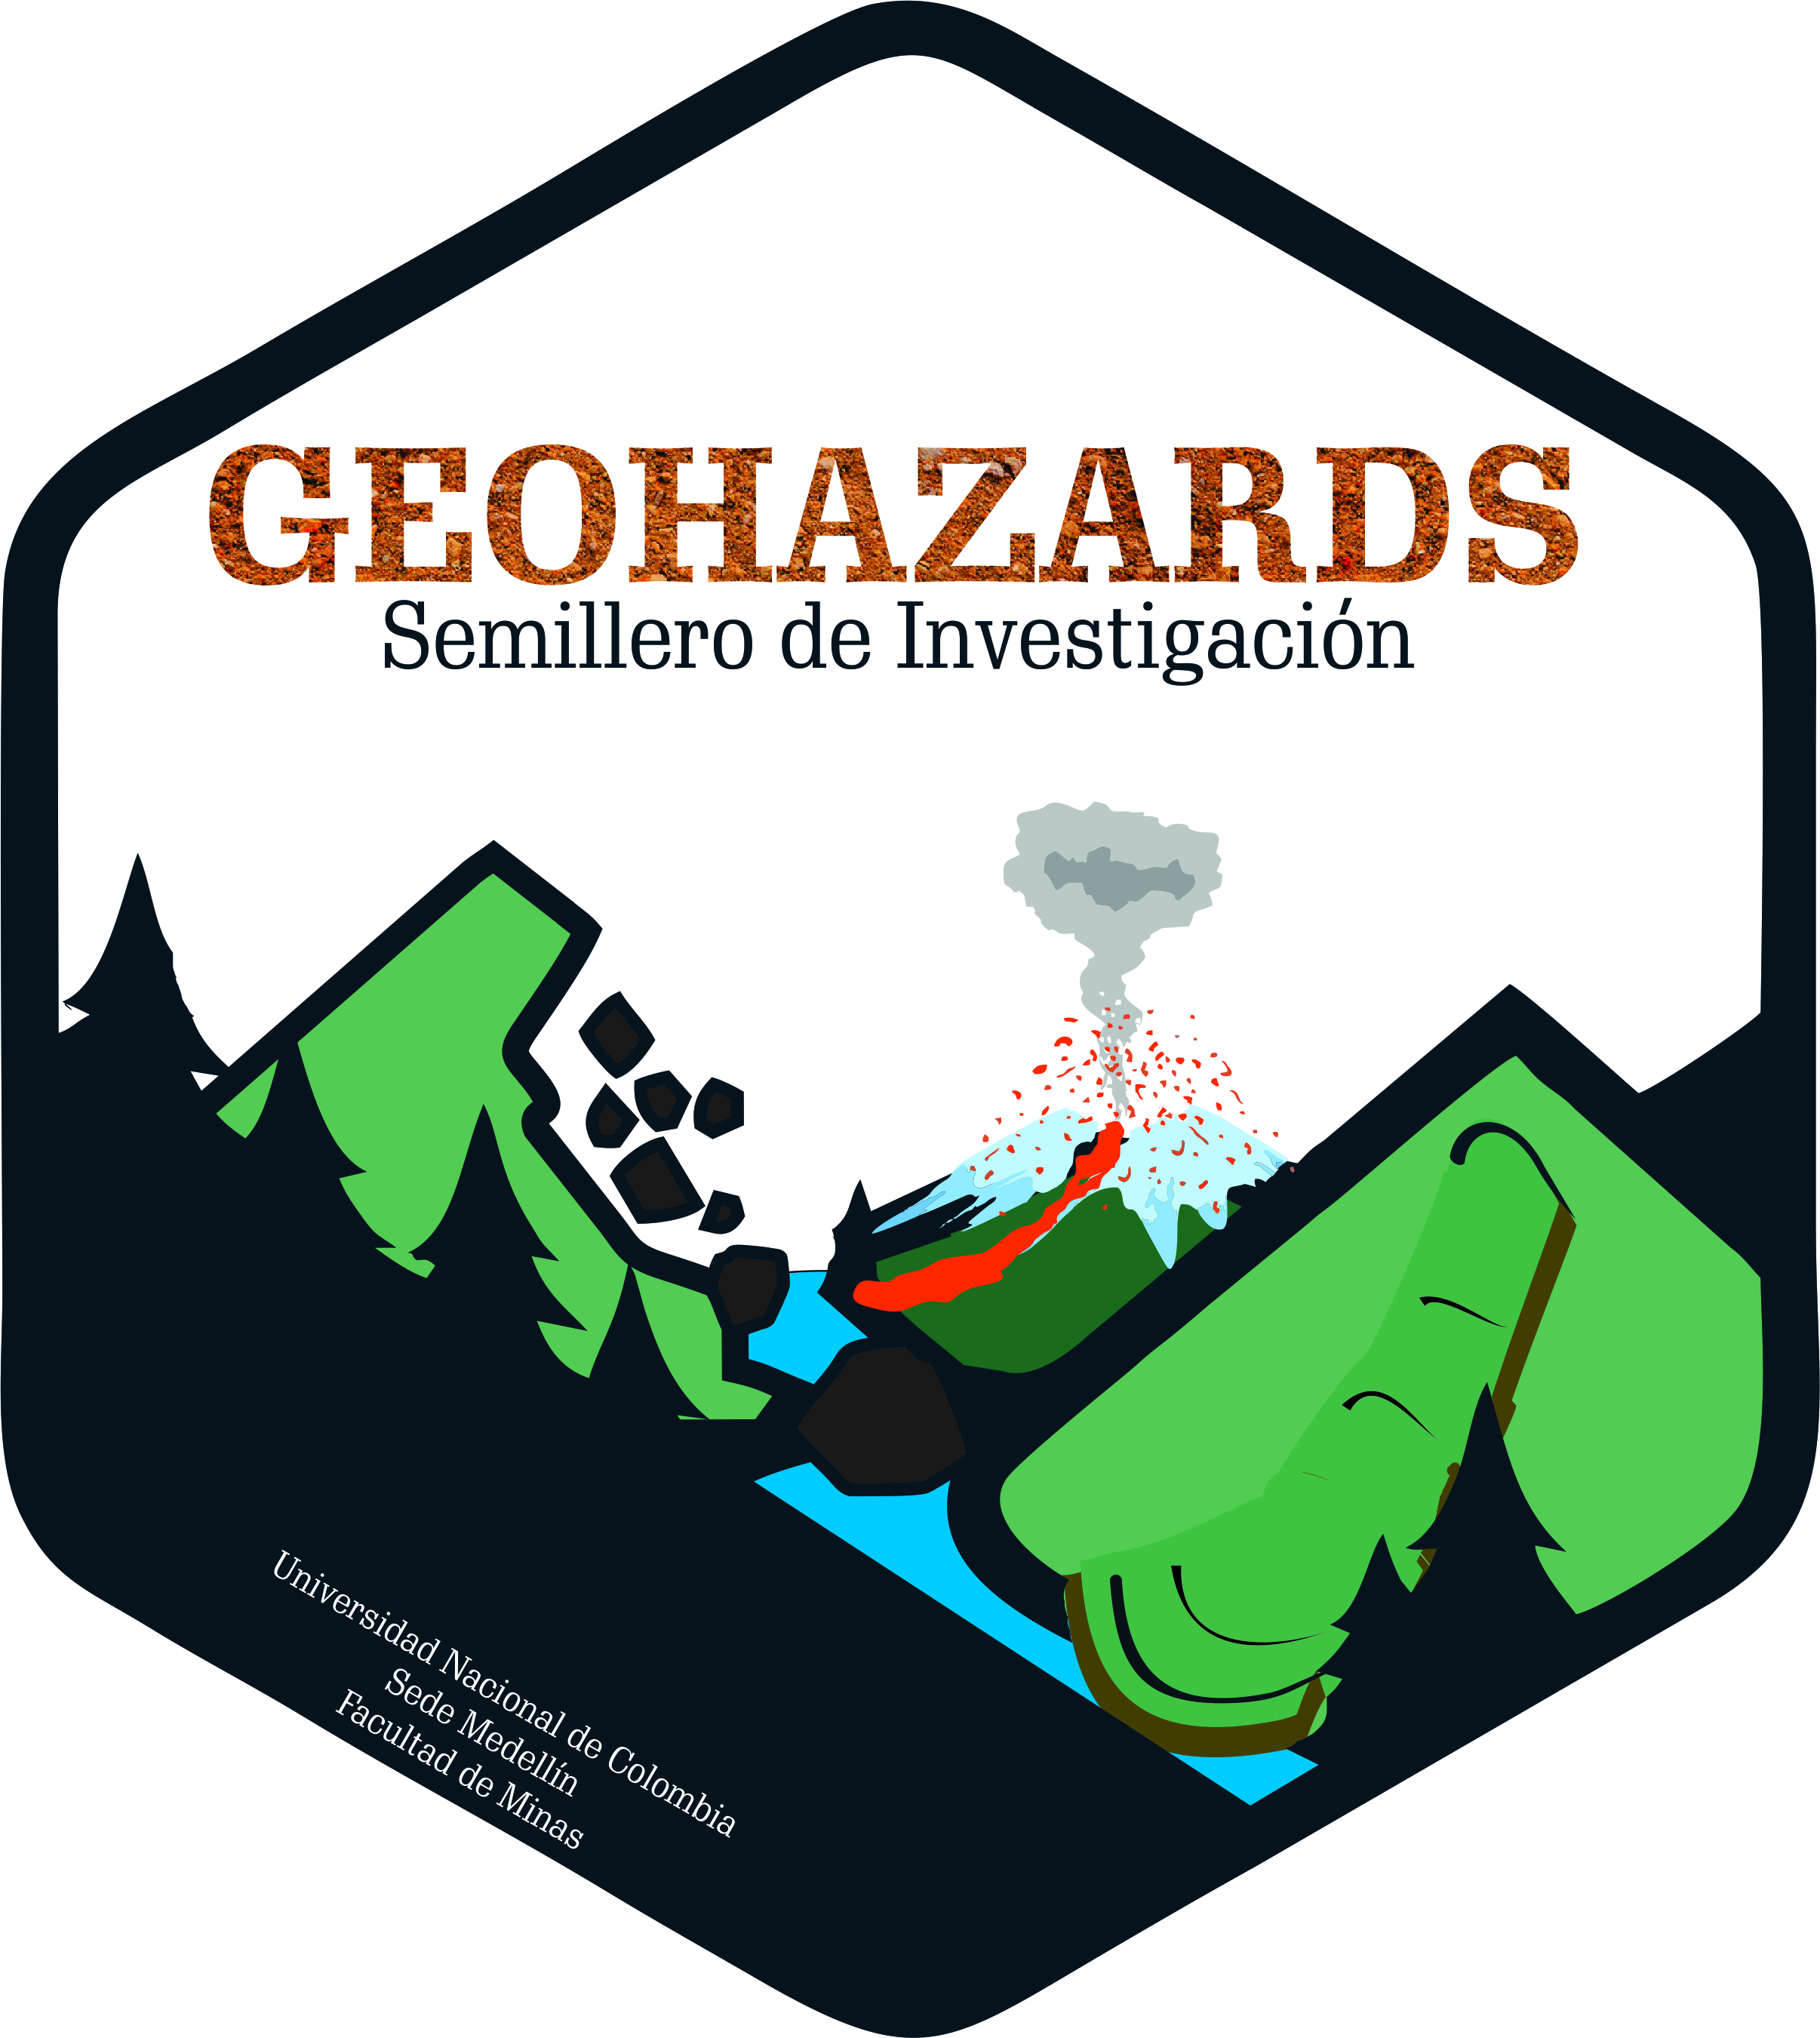
\includegraphics[height=1cm]{logo3}  
	\end{textblock*}
			}
%############################INICIO#############################################
\begin{document}
\begin{frame}
\titlepage
\centering
	
\includegraphics[width=5cm]{unal}\hspace*{4.75cm}~%
   	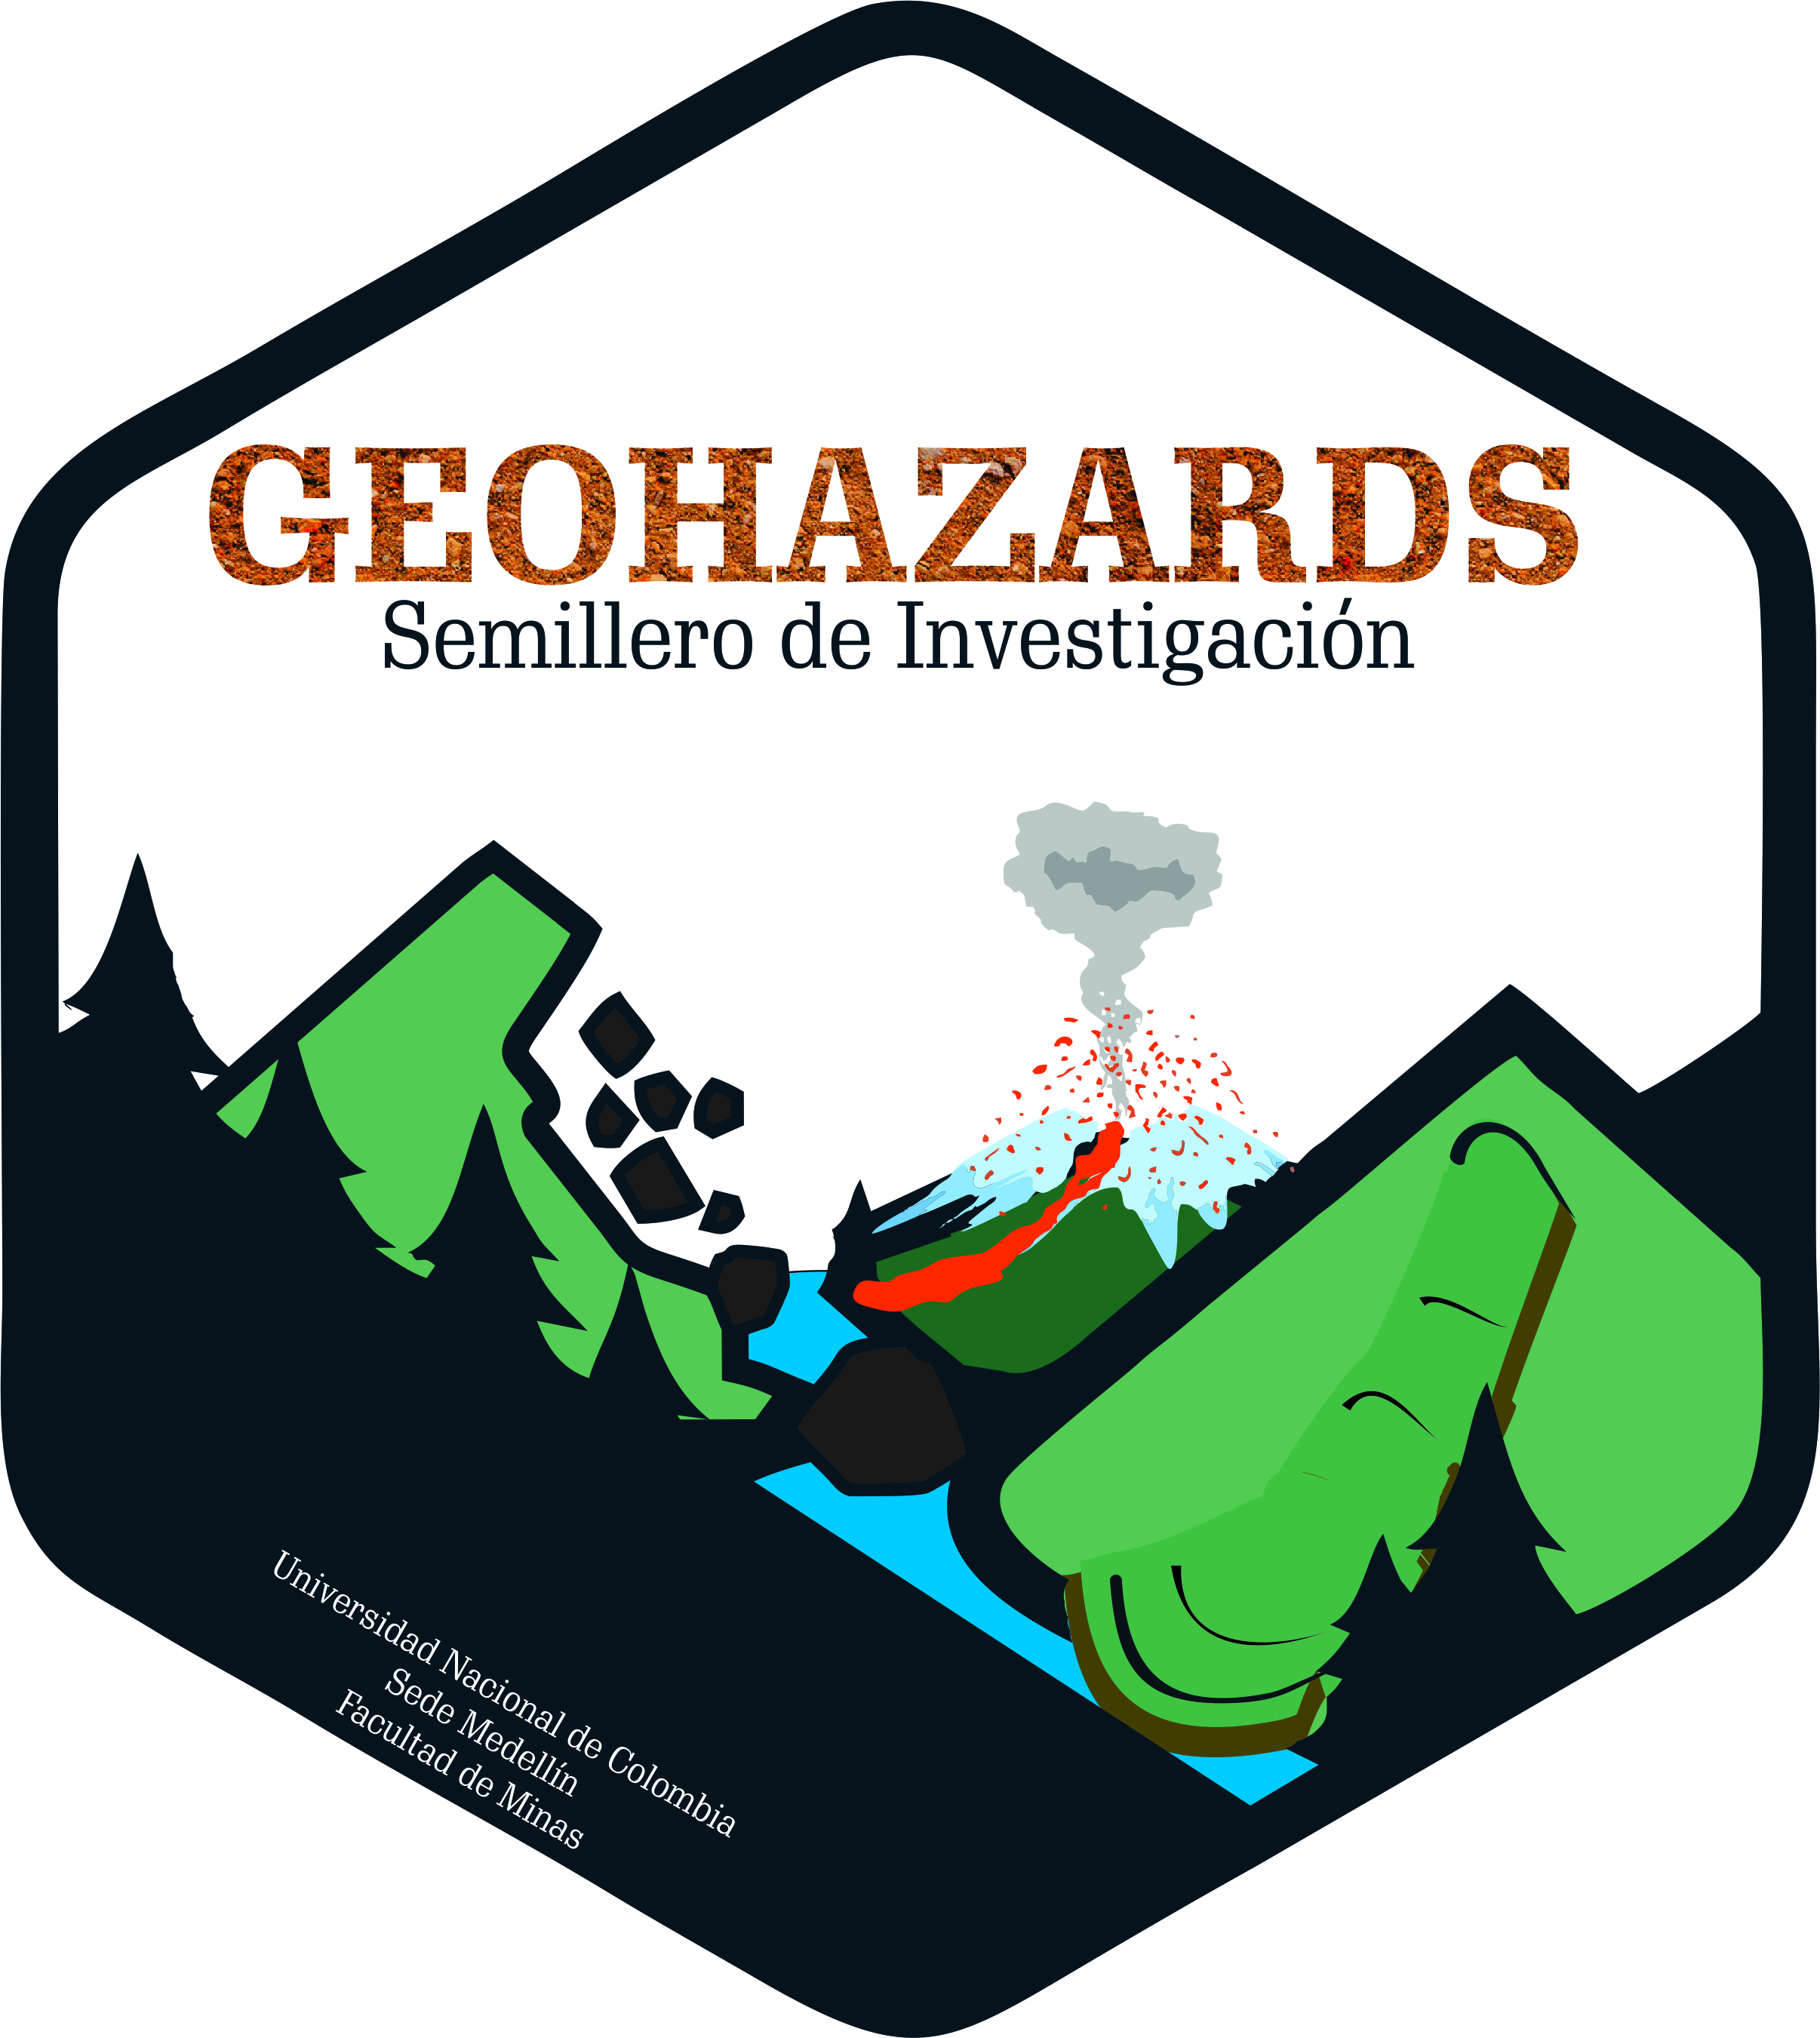
\includegraphics[width=2cm]{logo3} 
\end{frame}
 %#############################SLIDE
\begin{frame}
\frametitle{Sensores Remotos}
\scriptsize {Los \emph{Sensores Remotos} (teledetección) es el \textbf{arte, ciencia y tecnología} de observar un \textbf{objeto, escena o fenómeno} por técnicas basadas en instrumentos. El termino \emph{remoto} se refiere a la observación realizada a una distancia \textbf{sin contacto físico} con el objeto de interés. Se puede utilizar herramientas de detección y despliegue en tiempo real o una herramienta que registra la energía, la cual es emitida o reflejada desde el objeto o la escena en observación. La energía puede ser luz u otra forma de \textbf{radiaciones electromagnética}, campos de fuerza o energía acústica.}
\tiny{Fuente: ITC} 
  \begin{figure}
    \centering
    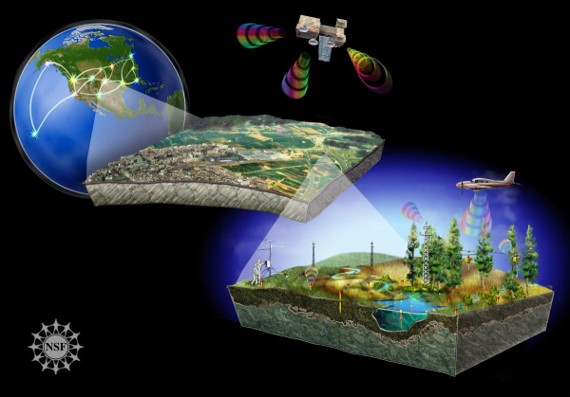
\includegraphics[height=.6\textheight]{definicion}
   \end{figure}
\end{frame}
%###############################SLIDE
\begin{frame}
  \begin{figure}
    \centering
    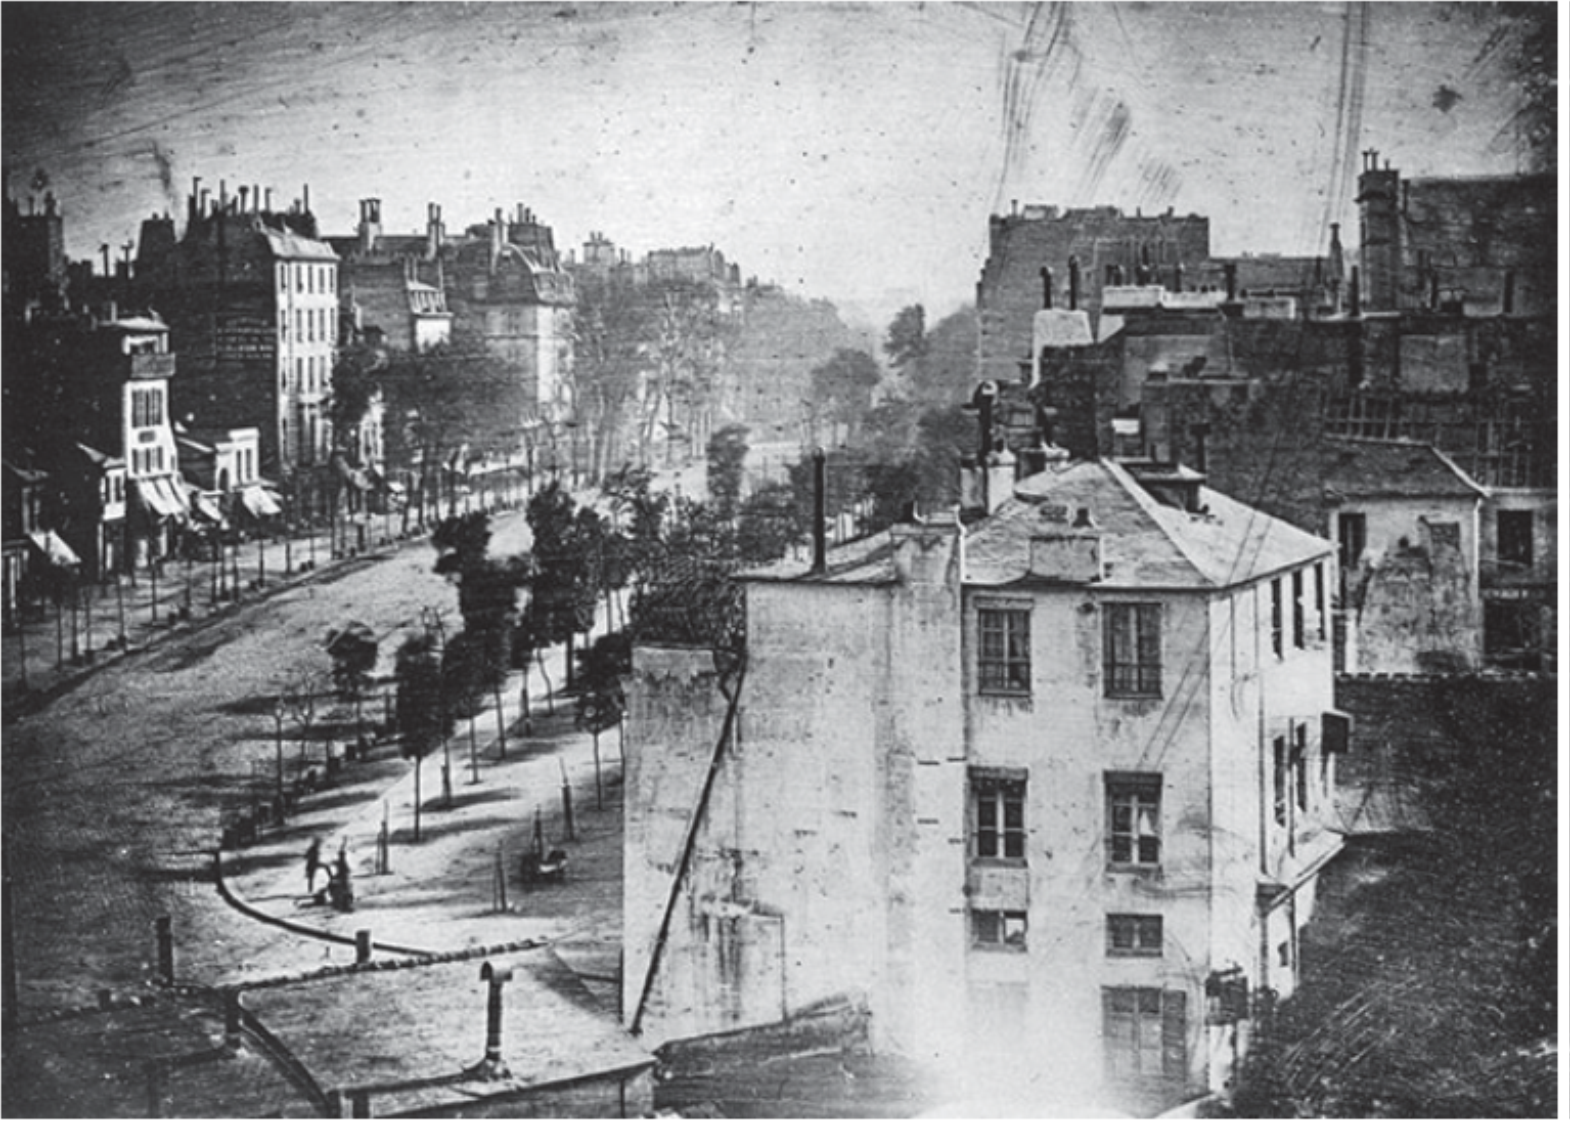
\includegraphics[height=.8\textheight]{G:/My Drive/CATEDRA/ANALISIS GEOESPACIAL/fig/foto1}
\tiny{}
 \end{figure}
\end{frame}
%################################SLIDE
\begin{frame}
  \begin{figure}
    \centering
    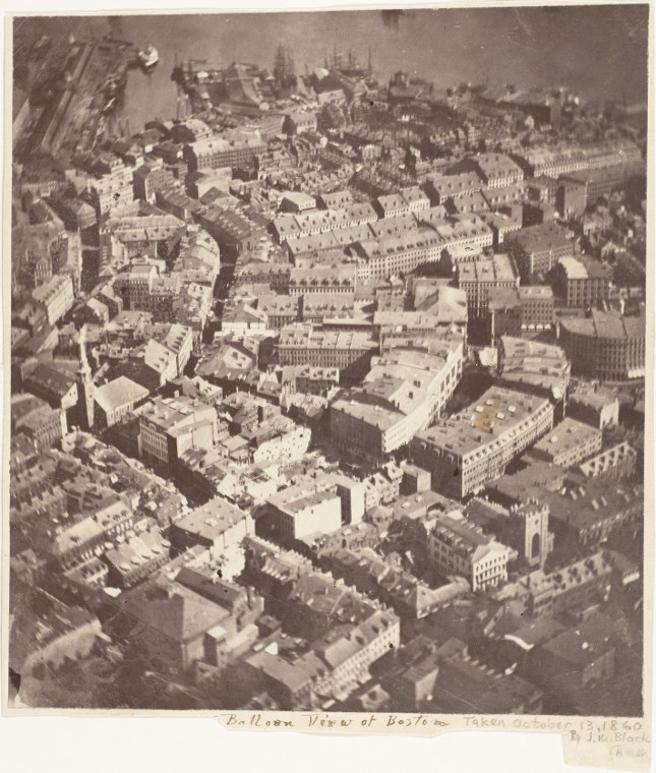
\includegraphics[height=.8\textheight]{G:/My Drive/CATEDRA/ANALISIS GEOESPACIAL/fig/boston}
\tiny{}
 \end{figure}
\end{frame}
%################################SLIDE
\begin{frame}
  \begin{figure}
    \centering
    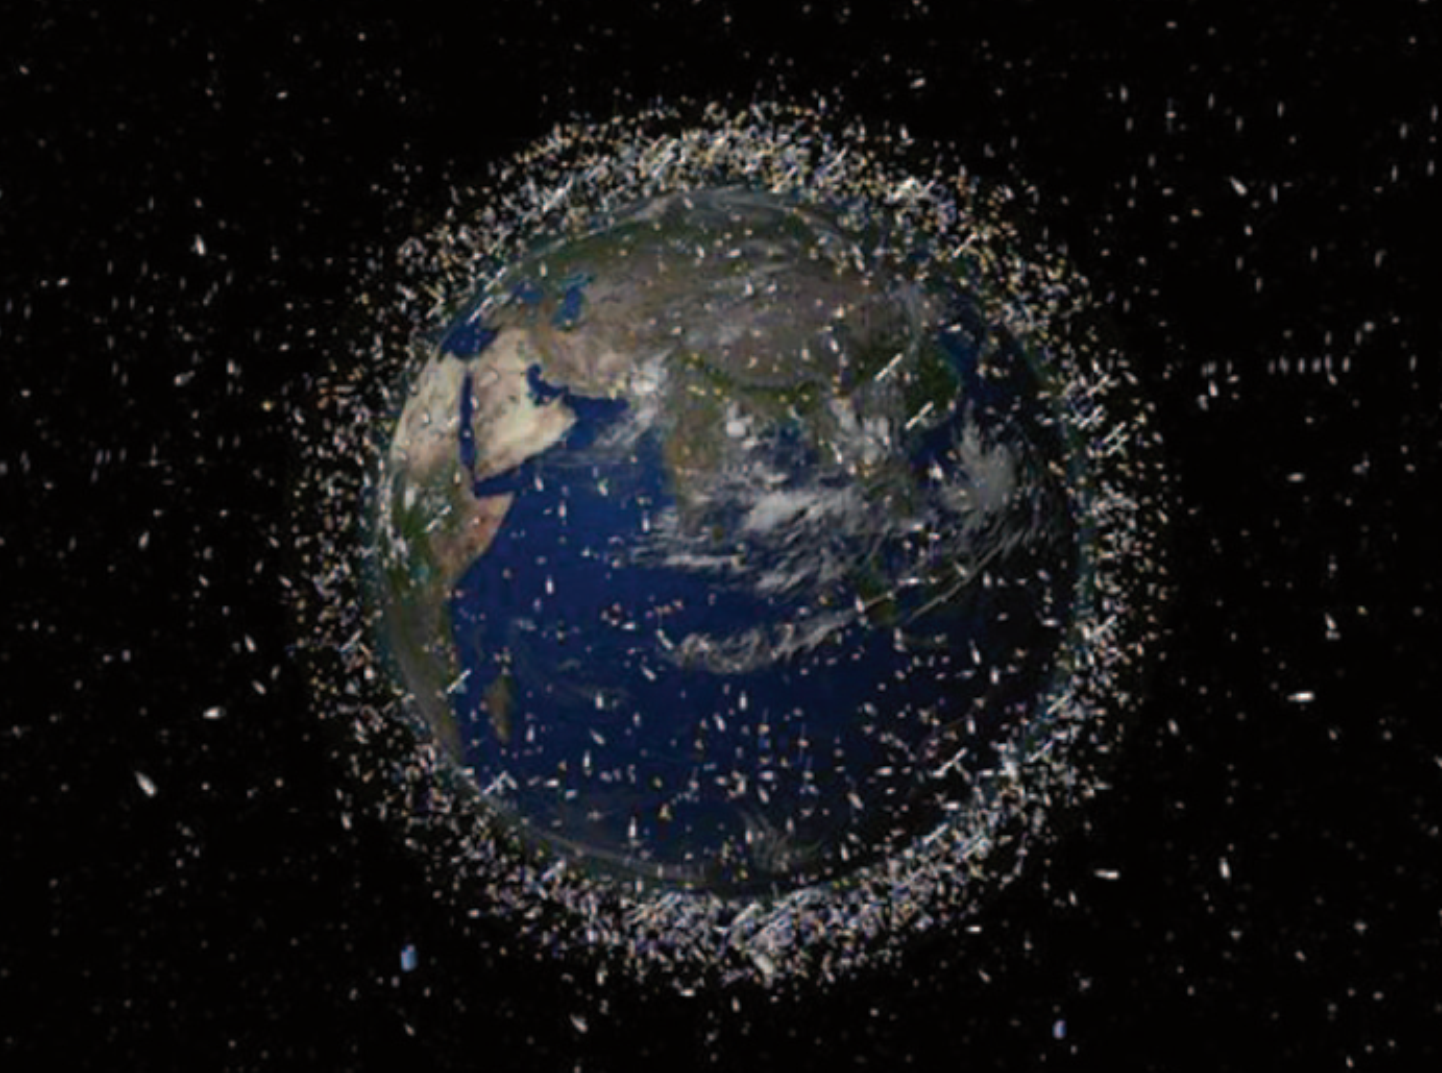
\includegraphics[height=.8\textheight]{G:/My Drive/CATEDRA/ANALISIS GEOESPACIAL/fig/satelite}
\tiny{}
 \end{figure}
\end{frame}
%################################SLIDE
\begin{frame}
\frametitle{Sensores Remotos}
  \begin{figure}
    \centering
    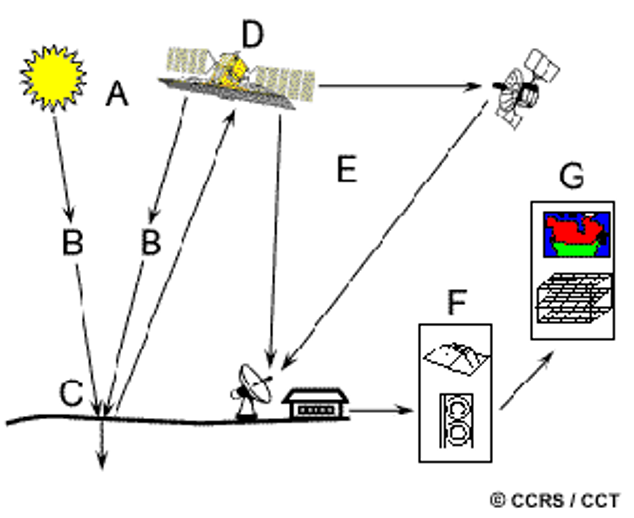
\includegraphics[height=.8\textheight]{G:/My Drive/CATEDRA/ANALISIS GEOESPACIAL/fig/bigpicture}
\tiny{}
 \end{figure}
\end{frame}
%################################SLIDE
\begin{frame}
\frametitle{Transferencia de Energía}
\scriptsize{Existen tres formas diferentes de transferencia energética en forma de calor}:
\begin{itemize}
\item \textbf{Conducción}: es el mecanismo de transferencia de calor en escala atómica. Se produce por la vibración y  choque de unas moléculas con otras, donde las partículas más energéticas le entregan energía a las menos energéticas.
\item \textbf{Convección}: mecanismo de transferencia de calor por movimiento de masa o circulación dentro de la sustancia, es propia de fluidos (líquidos o gaseosos) en movimiento.
\item \textcolor{red}{\textbf{Radiación}: es energía emitida por la materia que se encuentra a una temperatura dada. Esta energía es producida por los cambios en las configuraciones electrónicas de los átomos o moléculas. Esta energía es transportada por ondas electromagnéticas o fotones, por lo recibe el nombre de radiación electromagnética que se propaga a través del vacío y a la velocidad de la luz.}
\end{itemize}
\end{frame}
%################################SLIDE
\begin{frame}
\frametitle{Fuente de Energía}
\framesubtitle{Radiación Electromagnetica}
  \begin{figure}
    \centering
    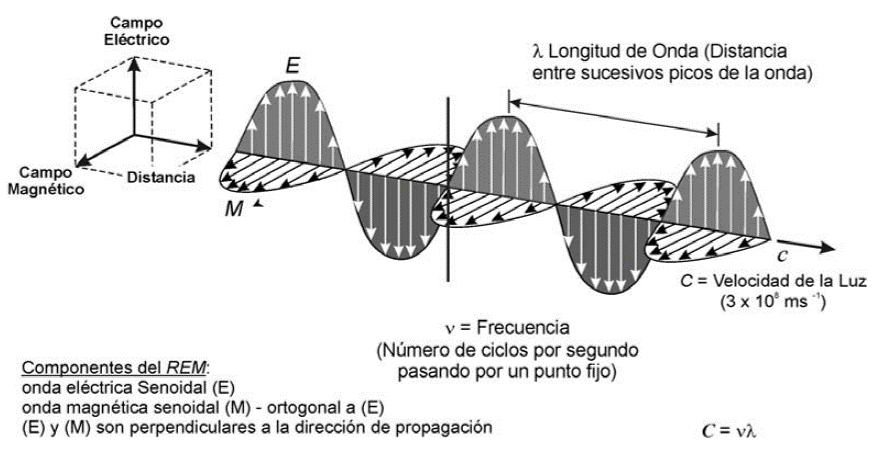
\includegraphics[height=.7\textheight]{G:/My Drive/CATEDRA/ANALISIS GEOESPACIAL/fig/wave}
\tiny{}
 \end{figure}
\end{frame}
%################################SLIDE
\begin{frame}
\frametitle{Wave-Particle Duality}
\framesubtitle{Young's experiment}
\begin{figure}
\centering
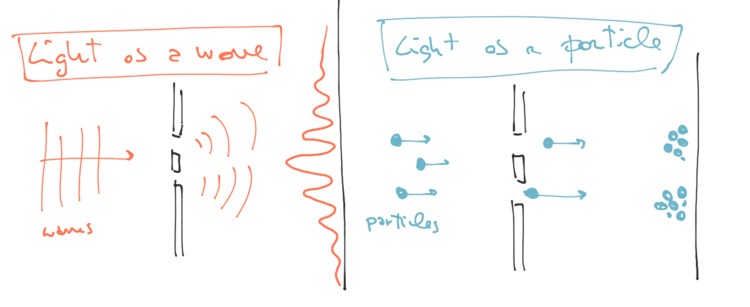
\includegraphics[width=10cm]{G:/My Drive/CATEDRA/ANALISIS GEOESPACIAL/fig/wave-particle}
\end{figure}
\begin{figure}
\centering
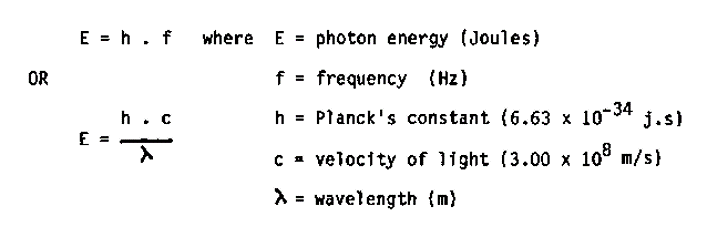
\includegraphics[width=8cm]{G:/My Drive/CATEDRA/ANALISIS GEOESPACIAL/fig/plank}
\end{figure}
\end{frame}
%###############################SLIDE
\begin{frame}
\frametitle{Espectro electromagnético}
  \begin{figure}
    \centering
    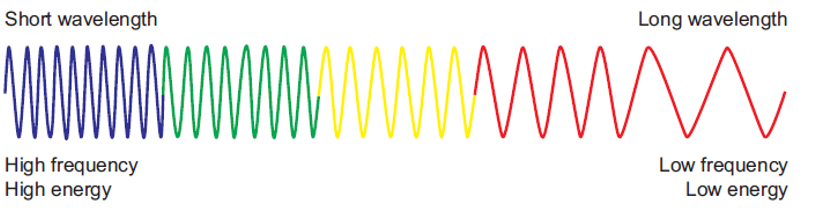
\includegraphics[height=.3\textheight]{G:/My Drive/CATEDRA/ANALISIS GEOESPACIAL/fig/wave2}
    %\caption{This is the caption.}
  \end{figure}
\end{frame}
%################################SLIDE
\begin{frame}
\frametitle{Fuente de Energía}
\framesubtitle{Ley de Stefan-Boltzmann \& Ley de Wien}
  \begin{figure}
    \centering
    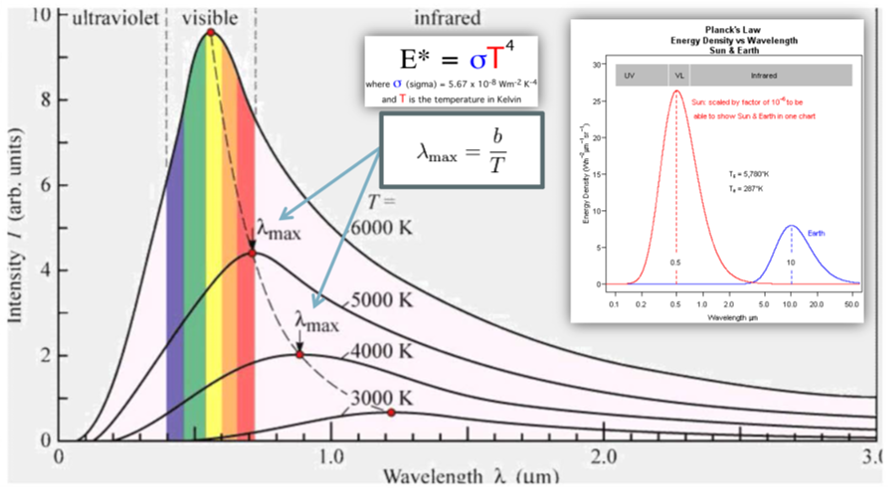
\includegraphics[height=.7\textheight]{G:/My Drive/CATEDRA/ANALISIS GEOESPACIAL/fig/stefan}
    %\caption{This is the caption.}
  \end{figure}
\end{frame}
%################################SLIDE
\begin{frame}
\frametitle{Espectro Electromagnético}
  \begin{figure}
    \centering
    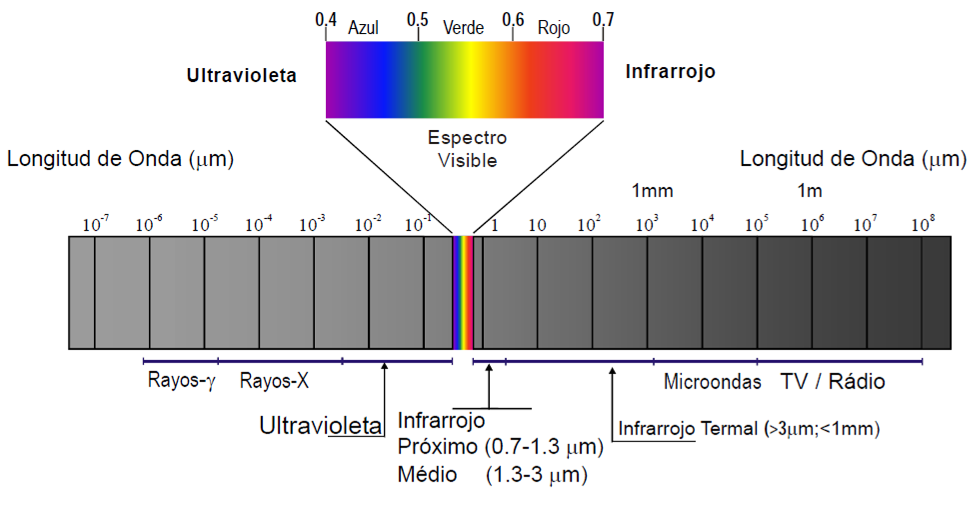
\includegraphics[height=.7\textheight]{G:/My Drive/CATEDRA/ANALISIS GEOESPACIAL/fig/espectro}
    %\caption{This is the caption.}
  \end{figure}
\end{frame}
%################################SLIDE
\begin{frame}
\frametitle{Espectro Electromagnético}
  \begin{figure}
    \centering
    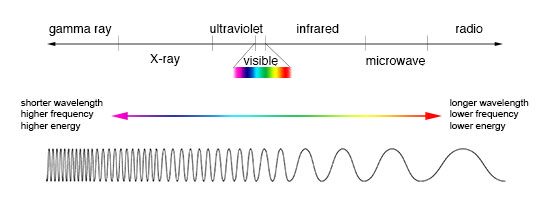
\includegraphics[height=.5\textheight]{espectro2}
  \end{figure}
\tiny{Credit: NASA's Imagine the Universe}
\end{frame}
%################################SLIDE
\begin{frame}
\begin{itemize}
\scriptsize{
\item \textbf{Energía radiante}: total de energía radiada en todas las direcciones (J).
\item \textbf{Flujo radiante}: energía radiada en todas las direcciones por unidad de tiempo (W).
\item \textbf{Irradiancia}: flujo radiante incidente sobre unidad de área ($\frac{w}{m^2}$).
\item \textbf{Radiancia}: flujo radiante emitido o reflejado por unidad de área y por ángulo solido de medida($\frac{w*Sr}{m^2}$).
\item \textbf{Emisividad}: relación entre la emitancia y la de un emisor perfecto.
\item \textbf{Reflectividad}: relación entre el flujo incidente y el flujo reflejado por una superficie.
\item \textbf{Absortividad}: relación entre el flujo incidente y el flujo que absorbe una superficie.
\item \textbf{Trasmisividad}: relación entre el flujo incidente y el transmitido por una superficie.
}
 \begin{figure}
    \centering
    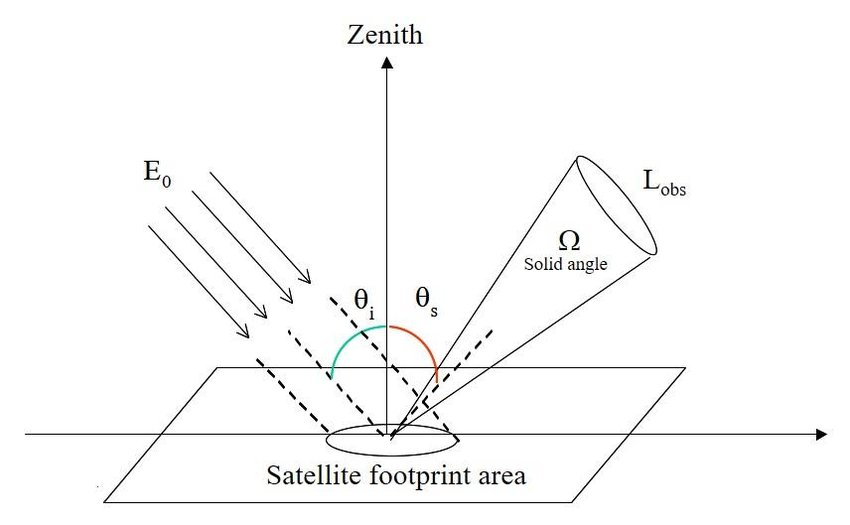
\includegraphics[height=.5\textheight]{G:/My Drive/CATEDRA/ANALISIS GEOESPACIAL/fig/radiance}
  \end{figure}
\end{itemize}
\end{frame}
%%%%%%%%%%%%%%%%%%%%%%%%%%%%%%%%%%%%%%%%%%%%%%%%%%%%%%%%%%%%
\begin{frame}
\frametitle{Interacción con la atmósfera}
%\framesubtitle{}
  \begin{figure}
    \centering
    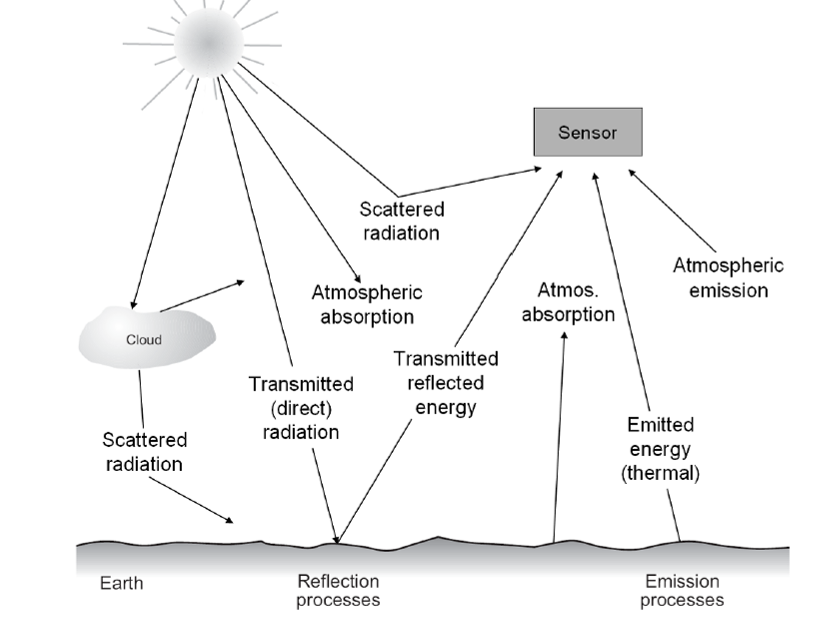
\includegraphics[height=.7\textheight]{G:/My Drive/CATEDRA/ANALISIS GEOESPACIAL/fig/atmosfera}
  \end{figure}
\end{frame}
%################################SLIDE
\begin{frame}
\frametitle{Atenuación}
  \begin{columns}
		\begin{column}{.4\linewidth}
		 \scriptsize{\textbf{Atenuación geométrica}: Atenuación de la radiación con la distancia recorrida desde la fuente hasta el receptor. La intensidad de la onda decrece usualmente con el cuadrado de la distancia al foco emisor.\\
\textbf{Atenuación atmosférica}: Atenuación por absorción de las moléculas atmosféricas. La intensidad de la onda disminuye exponencialmente con la distancia r del medio absorbente atravesado.}
		\end{column}
		\begin{column}{.6\linewidth}
			 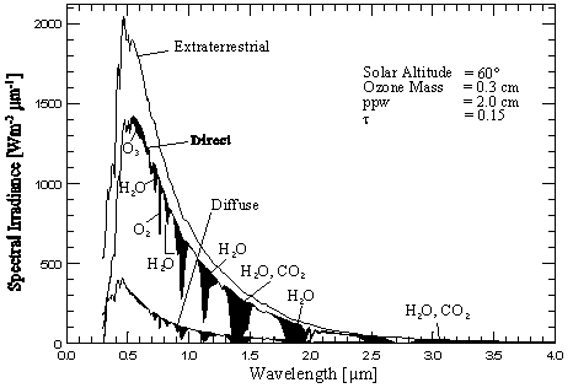
\includegraphics[height=.5\textheight]{G:/My Drive/CATEDRA/ANALISIS GEOESPACIAL/fig/atenuacion}
		\end{column}
	\end{columns}
\end{frame}
%################################SLIDE
\begin{frame}
\frametitle{Ventanas Atmosféricas}
\begin{center} 
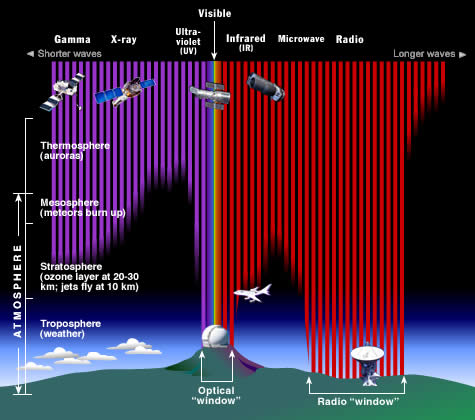
\includegraphics[width=8cm]{ventanas}
\end{center}
\tiny{Credit: NASA's Imagine the Universe}
\end{frame}
%################################SLIDE
\begin{frame}
\frametitle{Dispersión}
  \begin{columns}
		\begin{column}{.3\linewidth}
		 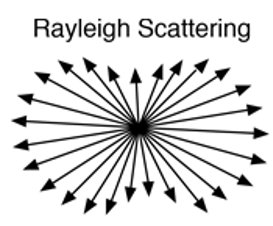
\includegraphics[width=3cm]{G:/My Drive/CATEDRA/ANALISIS GEOESPACIAL/fig/ray}
		\end{column}
		\begin{column}{.7\linewidth}
\scriptsize{\textbf{Rayleigh}: Dispersión dominante en la atmósfera. Diámetro de las partículas es inferior a la longitud de onda. Longitudes de ondas menores (azul) es mas disperso que longitudes de onda mayores (rojo). El efecto Rayleigh es inversamente proporcional a la longitud de onda a la 4. Se utilizan filtros que eliminan longitudes de onda corta.\\
(moléculas atmosféricas: O3, N2, CO2, etc)}.
		\end{column}
	\end{columns}
	\begin{columns}
		\begin{column}{.3\linewidth}
		 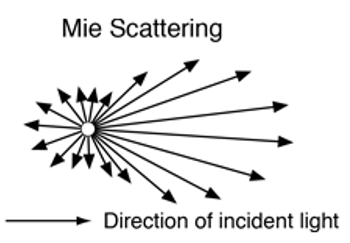
\includegraphics[width=4cm]{G:/My Drive/CATEDRA/ANALISIS GEOESPACIAL/fig/mie}
		\end{column}
		\begin{column}{.7\linewidth}
\scriptsize{\textbf{Mie}: Longitudes de onda similares al diámetro de las partículas, característico en la parte baja de la atmósfera. Mayor efecto en longitudes de onda mas grandes comparado con efecto Rayleigh.\\
(Polvo, Vapor de agua).}
		\end{column}
	\end{columns}
	\begin{columns}
	 	\begin{column}{.3\linewidth}
		 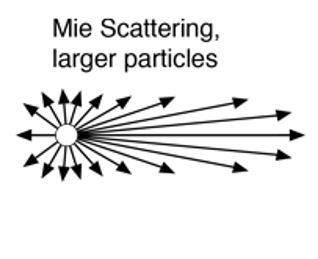
\includegraphics[width=4cm]{G:/My Drive/CATEDRA/ANALISIS GEOESPACIAL/fig/noselectiva}
		\end{column}
		\begin{column}{.7\linewidth}
\scriptsize{\textbf{No selectiva}. Diámetro (5  a 100 um) de las partículas es mucho mayor a las longitudes de onda, por lo que dispersa todo el espectro del visible y hasta el infrarrojo medio.\\
(Aerosoles, gotas de lluvia).}
		\end{column}
	\end{columns}
\end{frame}
%################################SLIDE
\begin{frame}
\frametitle{Interacción con el objeto}
  \begin{figure}
    \centering
    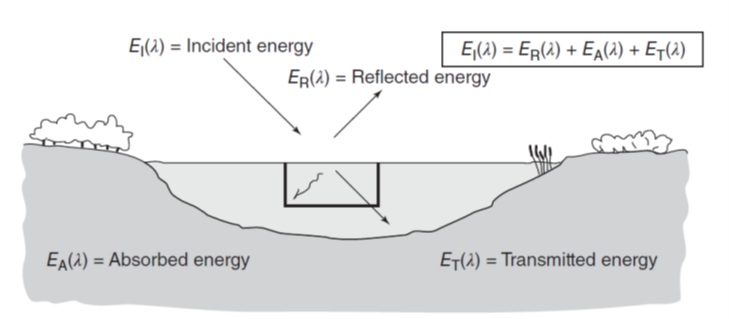
\includegraphics[height=.5\textheight]{G:/My Drive/CATEDRA/ANALISIS GEOESPACIAL/fig/objeto}
  \end{figure}
  \begin{columns}
	 	\begin{column}{.5\linewidth}
		 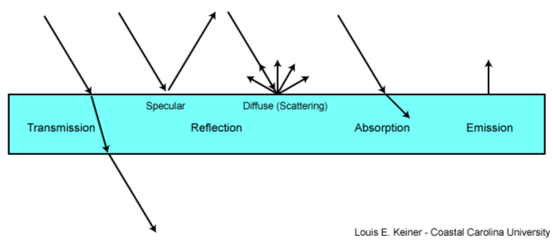
\includegraphics[width=5cm]{G:/My Drive/CATEDRA/ANALISIS GEOESPACIAL/fig/reflejo}
		\end{column}
		\begin{column}{.5\linewidth}
		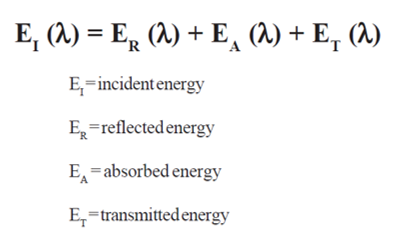
\includegraphics[width=4cm]{G:/My Drive/CATEDRA/ANALISIS GEOESPACIAL/fig/ecuacion}
		\end{column}
	\end{columns}
\tiny{}
\end{frame}
%################################SLIDE
\begin{frame}
\scriptsize{Se pueden distinguir dos tipos de superficies:\vfill\textbf{Especulares}. Aquellas que reflejan la energía con el mismo ángulo del flujo incidente.\vfill
\textbf{Lambertianas--difusa}.  Aquellas que reflejan el flujo incidente uniformemente en todas las direcciones. En Sensores Remotos generalmente es de mayor interés medir las propiedades de reflectancia difusa del terreno y objetos.} 
  \begin{figure}
    \centering
    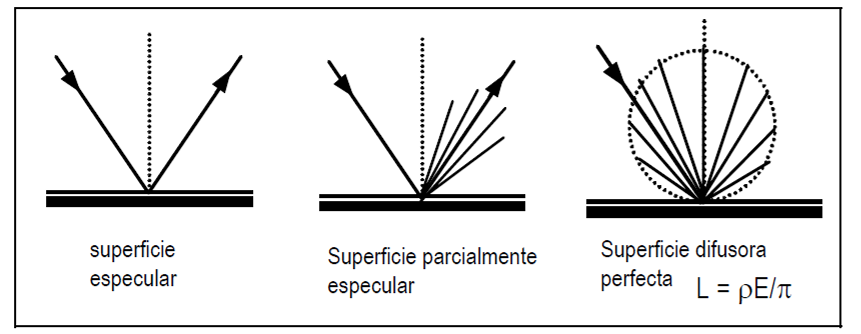
\includegraphics[height=.5\textheight]{G:/My Drive/CATEDRA/ANALISIS GEOESPACIAL/fig/objeto2}
  \end{figure}
\tiny{}
\end{frame}
%################################SLIDE
\begin{frame}
%\framesubtitle{}
  \begin{figure}
    \centering
    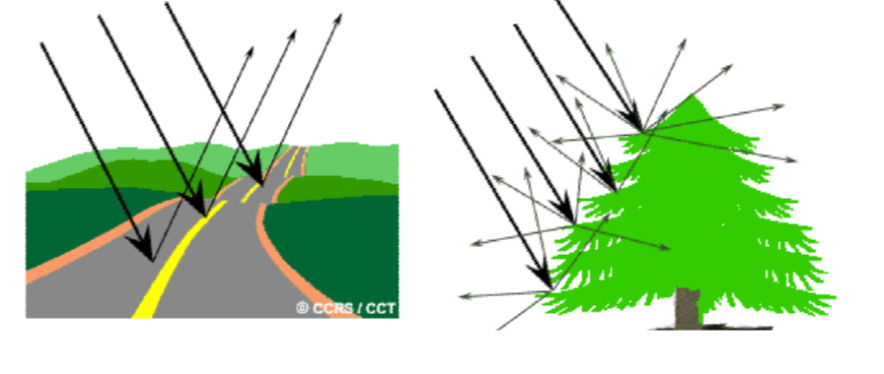
\includegraphics[height=.6\textheight]{G:/My Drive/CATEDRA/ANALISIS GEOESPACIAL/fig/dispersion2}
  \end{figure}
\end{frame}
%################################SLIDE
\begin{frame}
%\framesubtitle{}
  \begin{figure}
    \centering
    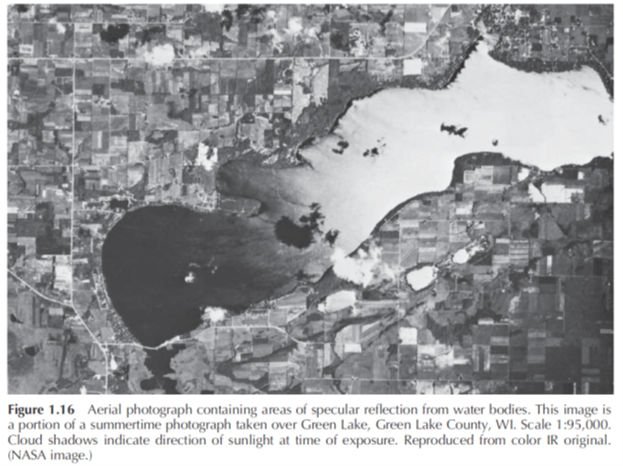
\includegraphics[height=.8\textheight]{G:/My Drive/CATEDRA/ANALISIS GEOESPACIAL/fig/especular}
  \end{figure}
\end{frame}
%################################SLIDE
\begin{frame}
\frametitle{Características de las coberturas}
\scriptsize{
La forma de reflejar la energía en las distintas longitudes de onda no es único y homogéneo, sino que varía sustancialmente en función de los siguientes factores:\vfill
\textbf{Físicos}: temperatura, humedad y textura.\vfill
\textbf{Químicos}: composición, contenido de materia orgánica, etc.\vfill
\textbf{Ambientales}: pendiente, orientación, estación del año, hora, etc.
}
 \begin{figure}
    \centering
    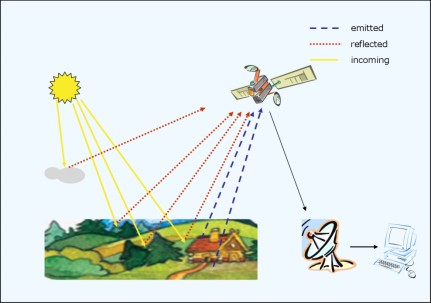
\includegraphics[height=.6\textheight]{G:/My Drive/CATEDRA/ANALISIS GEOESPACIAL/fig/paisaje}
  \end{figure}
\end{frame}
%%%%%%%%%%%%%%%%%%%%%%%%%%%%%%%%%%%%%%%%%%%%%%%%%%%%%%%%%%%%%%
\begin{frame}
  \begin{figure}
    \centering
    \subfloat[Angulo de iluminación solar\label{fig:a}]{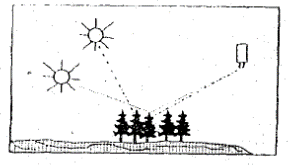
\includegraphics[width=4cm]{G:/My Drive/CATEDRA/ANALISIS GEOESPACIAL/fig/respuesta1}}\qquad
    \subfloat[Pendiente y orientación de las laderas\label{fig:b}]{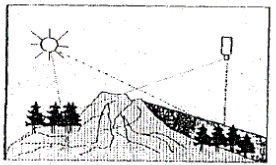
\includegraphics[width=4cm]{G:/My Drive/CATEDRA/ANALISIS GEOESPACIAL/fig/respuesta2}}
    \label{fig:1}
  \end{figure}
  \begin{figure}
    \centering
    \subfloat[Condiciones ambientales\label{fig:c}]{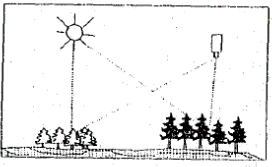
\includegraphics[width=4cm]{G:/My Drive/CATEDRA/ANALISIS GEOESPACIAL/fig/respuesta3}}\qquad    
    \subfloat[Condiciones atmosféricas\label{fig:d}]{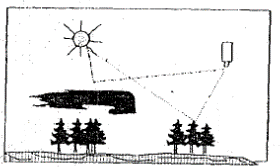
\includegraphics[width=4cm]{G:/My Drive/CATEDRA/ANALISIS GEOESPACIAL/fig/respuesta4}}
    \label{fig:2}
  \end{figure}
\end{frame}
%##############################SLIDE########################################### 
 \begin{frame}
\frametitle{Firma Espectral}
\scriptsize{La firma espectral se define como el comportamiento diferencial que presenta la radiación reflejada (reflectancia) o emitida (emitancia) desde algún tipo de superficie u objeto terrestre en los distintos rangos del espectro electromagnético. Una forma gráfica de estudiar este comportamiento es disponer los datos de reflectancia (\%) en el eje Y y la longitud de onda $\lambda$ en el eje X. Al unir los puntos con una línea continua se origina una representación bidimensional de la firma espectral}
 \begin{figure}
    \centering
    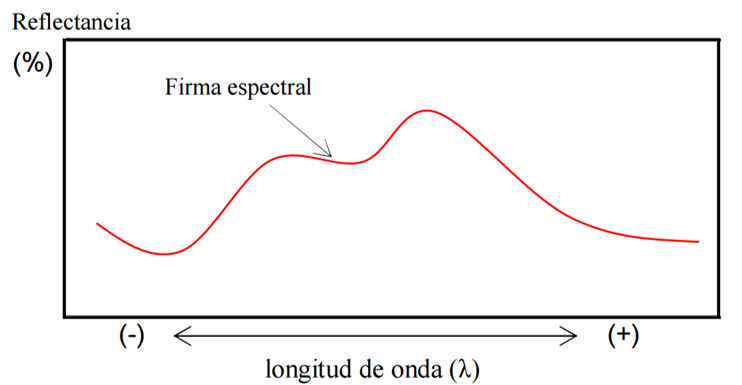
\includegraphics[height=.6\textheight]{G:/My Drive/CATEDRA/ANALISIS GEOESPACIAL/fig/firma}
  \end{figure}
\end{frame}
%%%%%%%%%%%%%%%%%%%%%%%%%%%%%%%%%%%%%%%%%%%%%%%%%%%%%%%%%%%%%%
\begin{frame}
%\framesubtitle{}
  \begin{figure}
    \centering
    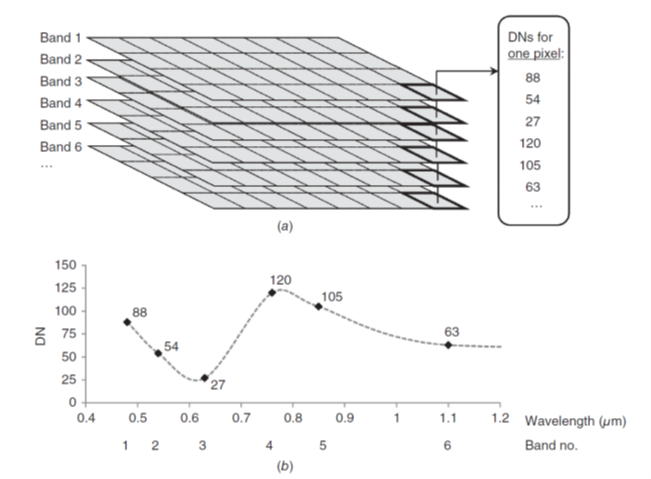
\includegraphics[height=.8\textheight]{G:/My Drive/CATEDRA/ANALISIS GEOESPACIAL/fig/firma2}
  \end{figure}
\end{frame}
%################################SLIDE
\begin{frame}
%\framesubtitle{}
  \begin{figure}
    \centering
    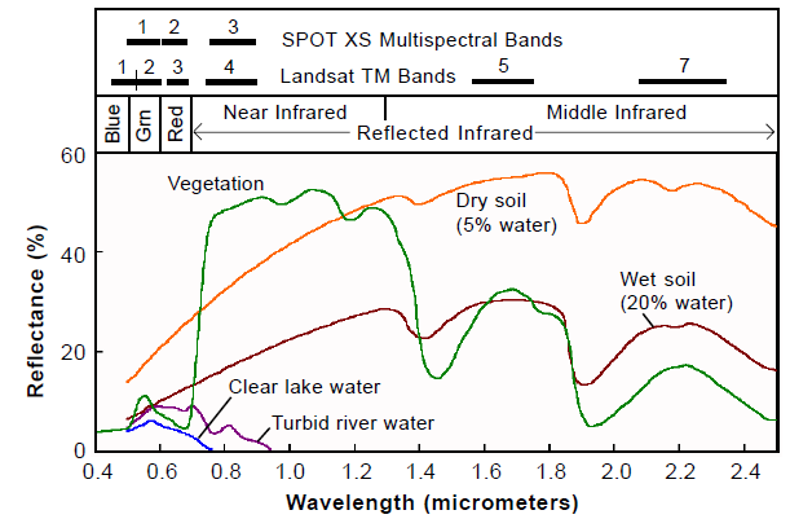
\includegraphics[height=.8\textheight]{G:/My Drive/CATEDRA/ANALISIS GEOESPACIAL/fig/firma3}
  \end{figure}
\end{frame}
%################################SLIDE
\begin{frame}
\frametitle{Vegetación}
  \begin{figure}
    \centering
    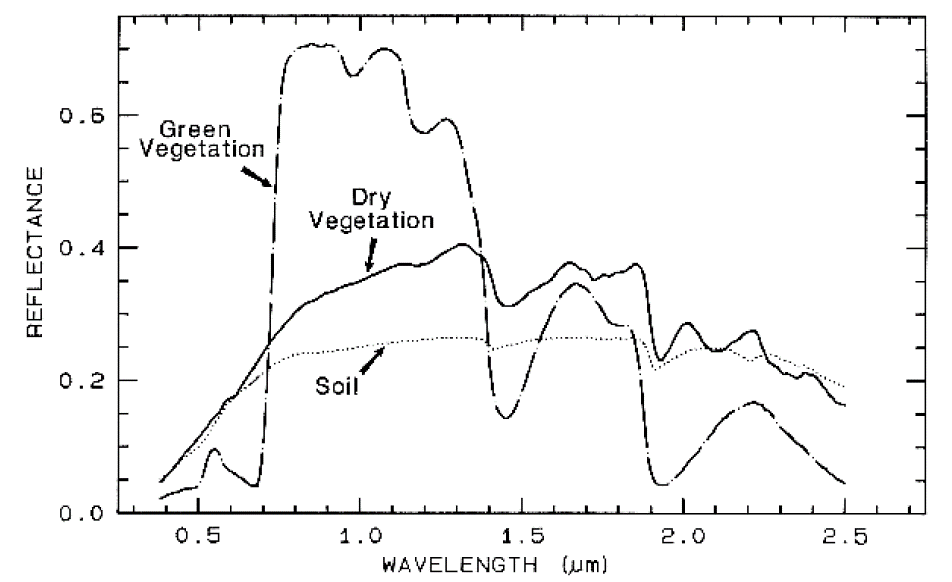
\includegraphics[height=.8\textheight]{G:/My Drive/CATEDRA/ANALISIS GEOESPACIAL/fig/firma4}
  \end{figure}
\end{frame}
%################################SLIDE
\begin{frame}
\frametitle{Agua \& Sedimentos}
  \begin{figure}
    \centering
    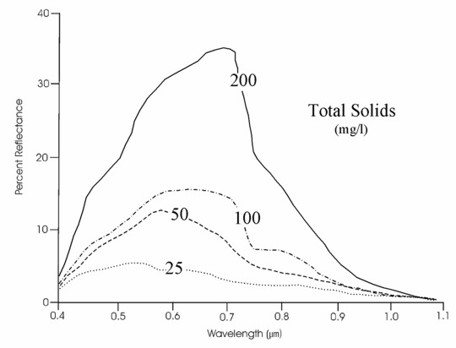
\includegraphics[height=.8\textheight]{G:/My Drive/CATEDRA/ANALISIS GEOESPACIAL/fig/firma5}
  \end{figure}
\end{frame}
%################################SLIDE
\begin{frame}
\frametitle{Suelo \& Humedad}
  \begin{figure}
    \centering
    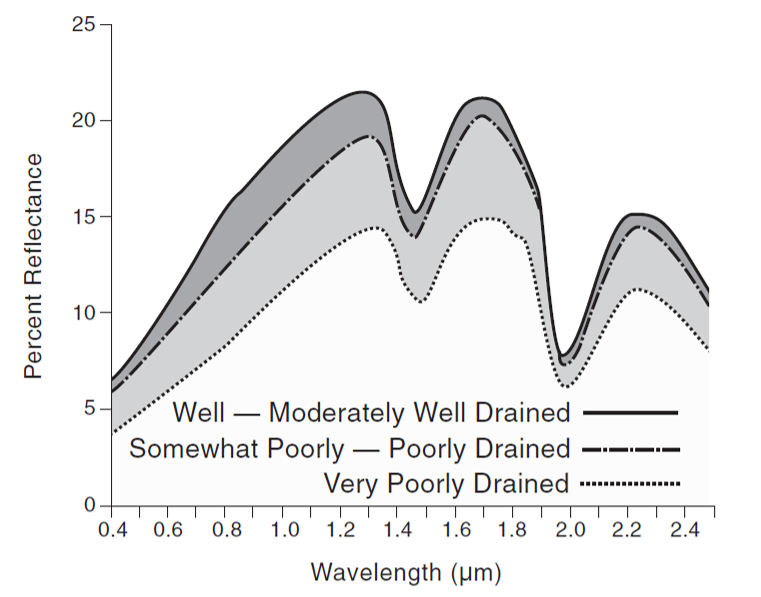
\includegraphics[height=.8\textheight]{G:/My Drive/CATEDRA/ANALISIS GEOESPACIAL/fig/firma6}
  \end{figure}
\end{frame}
%################################SLIDE
\begin{frame}
\frametitle{Suelo \& Granulometría}
  \begin{figure}
    \centering
    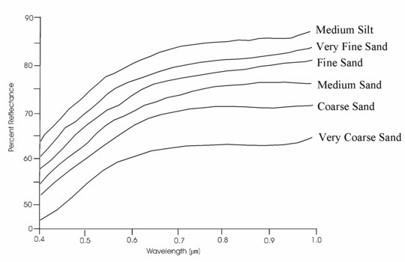
\includegraphics[height=.8\textheight]{G:/My Drive/CATEDRA/ANALISIS GEOESPACIAL/fig/firma7}
  \end{figure}
\end{frame}
%################################SLIDE
\begin{frame}
\frametitle{Sensores}
  \begin{figure}
    \centering
    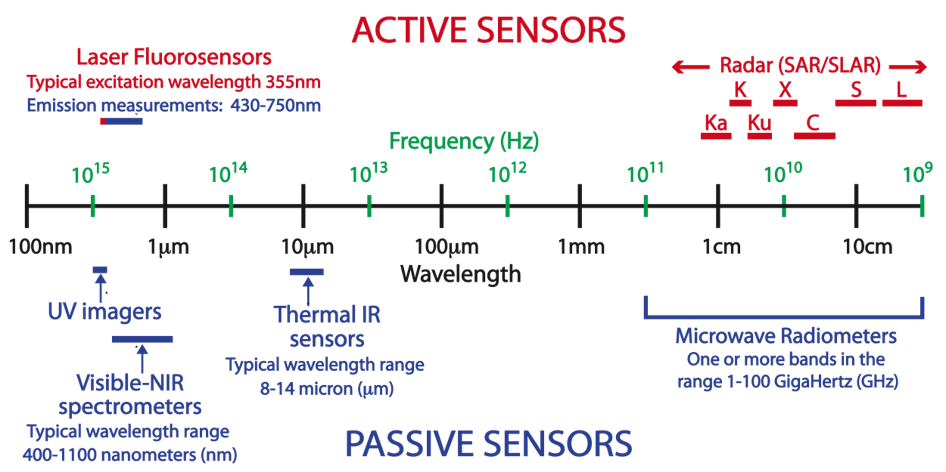
\includegraphics[height=.7\textheight]{G:/My Drive/CATEDRA/ANALISIS GEOESPACIAL/fig/activospasivos}
  \end{figure}
\end{frame}
%################################SLIDE
 \begin{frame}
\frametitle{Orbitas}
\scriptsize{
\textbf{Altitud}: distancia desde el satélite a la superficie de la tierra. A mayor altitud menor resolución espacial.\\
\textbf{Angulo de inclinación}:  ángulo entre el plano de la orbita y el plano ecuatorial. Determina la porción de tierra que observa.\\
\textbf{Periodo}: es el tiempo que requiere para completar una orbita. La velocidad afecta la resolución, si aumenta al velocidad se reduce la exposición y se requiere alta intensidad de radiación.\\
\textbf{Ciclo repetido}: es el tiempo entre dos sucesivas orbitas idénticas.
}
 \begin{figure}
    \centering
    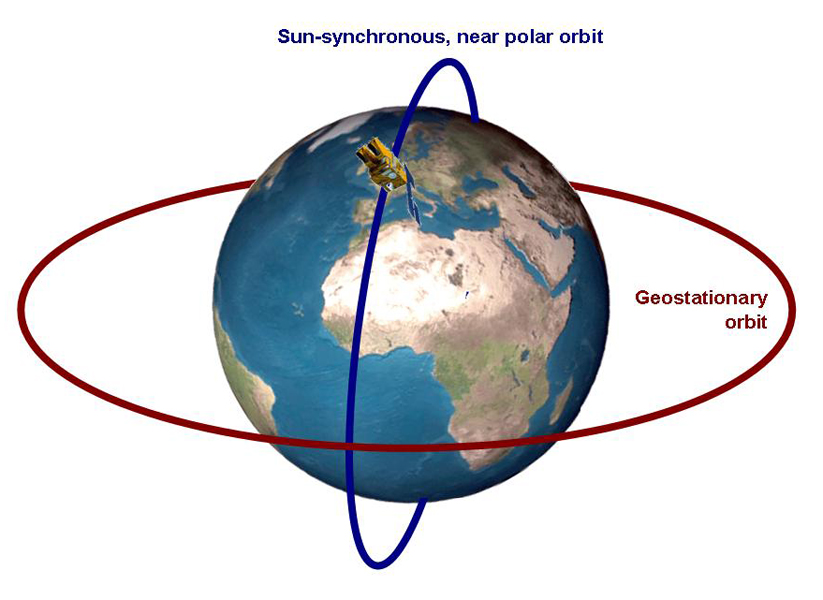
\includegraphics[height=.6\textheight]{G:/My Drive/CATEDRA/ANALISIS GEOESPACIAL/fig/orbitas}
  \end{figure}
\end{frame}
%%%%%%%%%%%%%%%%%%%%%%%%%%%%%%%%%%%%%%%%%%%%%%%%%%%%%%%%%%%%%%
\begin{frame}
\frametitle{Swaths} 
\scriptsize{
\textbf{Swath}: El área que cubre el sensor de cierta porción de la tierra. Puede variar de diez a cientos de kilómetros de ancho. Debido a la rotación de la tierra le permite al satélite cubrir una nueva área en cada paso consecutivo.
}
 \begin{figure}
    \centering
    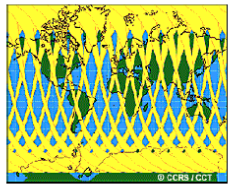
\includegraphics[height=.6\textheight]{G:/My Drive/CATEDRA/ANALISIS GEOESPACIAL/fig/swaths}
  \end{figure}
\end{frame}
%%%%%%%%%%%%%%%%%%%%%%%%%%%%%%%%%%%%%%%%%%%%%%%%%%%%%%%%%%%%%%
\begin{frame}
\frametitle{Landsat 8}
 \begin{figure}
    \centering
    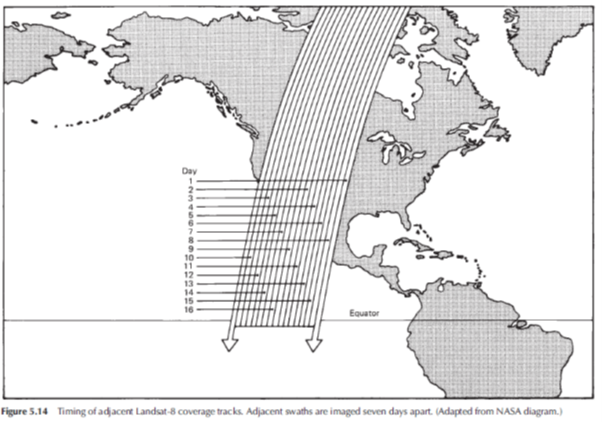
\includegraphics[height=.8\textheight]{G:/My Drive/CATEDRA/ANALISIS GEOESPACIAL/fig/swaths8}
  \end{figure}
\end{frame}
%%%%%%%%%%%%%%%%%%%%%%%%%%%%%%%%%%%%%%%%%%%%%%%%%%%%%%%%%%%%%%
 \begin{frame}
\frametitle{Polares \& Heliosincrónicas}
\scriptsize{
\textbf{Orbitas polares}: pasan por los polos de la tierra, con inclinación entre 80 y 100 °. Cubrimiento del planeta, mayor escala espacial (m).\vfill
\textbf{Sincrónica al Sol (heliosincrónica)}: orbita en la cual el satélite siempre pasa un área en el mismo tiempo, y permite tomas imágenes de noche en la fase ascendente (termal o radar). LANDSAT, SPOT e IRIS.
}
 \begin{figure}
    \centering
    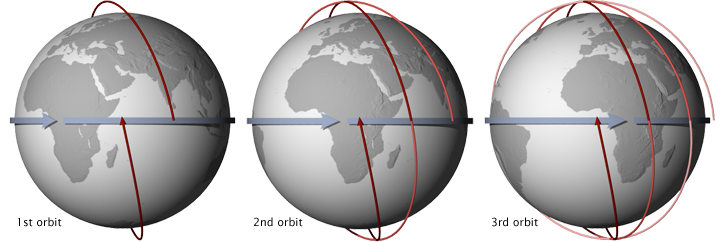
\includegraphics[height=.4\textheight]{G:/My Drive/CATEDRA/ANALISIS GEOESPACIAL/fig/polar}
  \end{figure}
\end{frame}
%%%%%%%%%%%%%%%%%%%%%%%%%%%%%%%%%%%%%%%%%%%%%%%%%%%%%%%%%%%%%%
 \begin{frame}
\frametitle{Geosincrónica \& Geoestacionaria}
\scriptsize{
\textbf{Orbitas ecuatoriales}: donde el satélite está localizado sobre el ecuador, ángulo de inclinación 0° y a 36k km.\vfill
\textbf{Geoestacionarias}: el satélite está en una posición relativa fija sobre la tierra. Menor escala espacial (Km) pero mayor resolución temporal.
}
 \begin{figure}
    \centering
    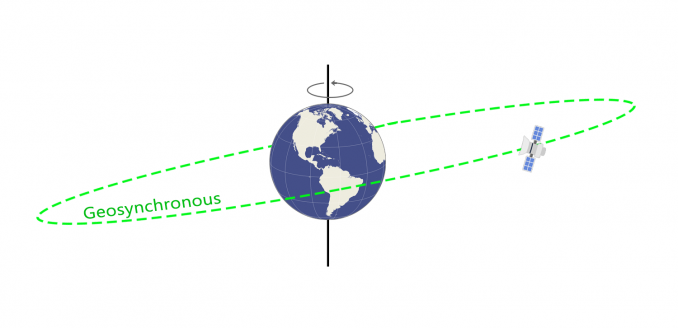
\includegraphics[height=.6\textheight]{G:/My Drive/CATEDRA/ANALISIS GEOESPACIAL/fig/ecuador}
  \end{figure}
\end{frame}
%%%%%%%%%%%%%%%%%%%%%%%%%%%%%%%%%%%%%%%%%%%%%%%%%%%%%%%%%%%%%%
\begin{frame}
\frametitle{Plataformas} 
 \begin{figure}
    \centering
    \includegraphics[height=.8\textheight]{G:/My Drive/CATEDRA/ANALISIS GEOESPACIAL/fig/plataforma}
  \end{figure}
\end{frame}
%%%%%%%%%%%%%%%%%%%%%%%%%%%%%%%%%%%%%%%%%%%%%%%%%%%%%%%%%%%%%%
\begin{frame}
\frametitle{Satélite Bus}
  \begin{columns}
		\begin{column}{.5\linewidth}
		 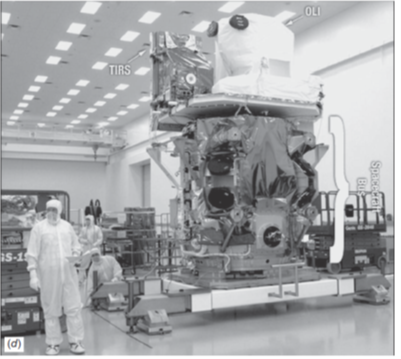
\includegraphics[width=6cm]{G:/My Drive/CATEDRA/ANALISIS GEOESPACIAL/fig/landsat2}
		\end{column}
		\begin{column}{.5\linewidth}
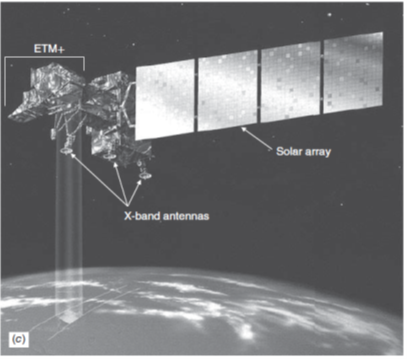
\includegraphics[width=6cm]{G:/My Drive/CATEDRA/ANALISIS GEOESPACIAL/fig/landsat3}
		\end{column}
	\end{columns}
\end{frame}
%%%%%%%%%%%%%%%%%%%%%%%%%%%%%%%%%%%%%%%%%%%%%%%%%%%%%%%%%%%%%%%
\begin{frame}
\frametitle{Sensores} 
 \begin{figure}
    \centering
    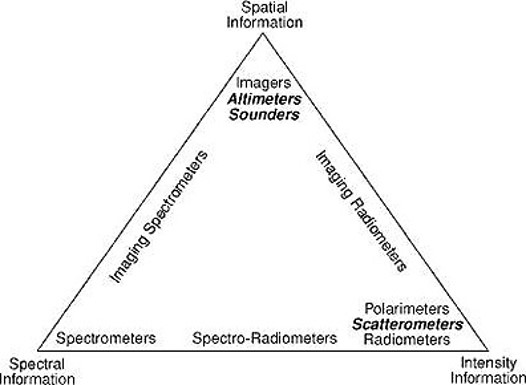
\includegraphics[height=.8\textheight]{G:/My Drive/CATEDRA/ANALISIS GEOESPACIAL/fig/sensores}
  \end{figure}
\end{frame}
%%%%%%%%%%%%%%%%%%%%%%%%%%%%%%%%%%%%%%%%%%%%%%%%%%%%%%%%%%%%%%
\begin{frame}
\frametitle{Detectores}
  \begin{columns}
		\begin{column}{.3\linewidth}
		 \includegraphics[width=4cm]{G:/My Drive/CATEDRA/ANALISIS GEOESPACIAL/fig/detector}
		\end{column}
		\begin{column}{.7\linewidth}
\includegraphics[width=8cm]{G:/My Drive/CATEDRA/ANALISIS GEOESPACIAL/fig/pixel}
		\end{column}
	\end{columns}
\end{frame}
%%%%%%%%%%%%%%%%%%%%%%%%%%%%%%%%%%%%%%%%%%%%%%%%%%%%%%%%%%%%%%
\begin{frame}
\frametitle{Detectores Cuánticos}
\scriptsize{
Los detectores son definidos como instrumentos que reciben un flujo de energía y proporcionan una señal. Existen dos tipos fundamentales de detectores de luz que operan con mecanismos de transducción diferentes.
}
 \begin{figure}
    \centering
    \includegraphics[height=.6\textheight]{G:/My Drive/CATEDRA/ANALISIS GEOESPACIAL/fig/ccd}
  \end{figure}
\end{frame}
%%%%%%%%%%%%%%%%%%%%%%%%%%%%%%%%%%%%%%%%%%%%%%%%%%%%%%%%%%%%%%
\begin{frame}
\frametitle{Detectores Térmicos}
\scriptsize{
Los detectores son definidos como instrumentos que reciben un flujo de energía y proporcionan una señal. Existen dos tipos fundamentales de detectores de luz que operan con mecanismos de transducción diferentes.
}
  \begin{columns}
		\begin{column}{.5\linewidth}
		 \includegraphics[width=6cm]{G:/My Drive/CATEDRA/ANALISIS GEOESPACIAL/fig/termal2}
		\end{column}
		\begin{column}{.5\linewidth}
\includegraphics[width=6cm]{G:/My Drive/CATEDRA/ANALISIS GEOESPACIAL/fig/termal3}
		\end{column}
	\end{columns}
\end{frame}
%%%%%%%%%%%%%%%%%%%%%%%%%%%%%%%%%%%%%%%%%%%%%%%%%%%%%%%%%%%%%%
\begin{frame}
\frametitle{Análoga vs Scanning} 
 \begin{figure}
    \centering
    \includegraphics[height=.8\textheight]{G:/My Drive/CATEDRA/ANALISIS GEOESPACIAL/fig/frame}
  \end{figure}
\end{frame}
%%%%%%%%%%%%%%%%%%%%%%%%%%%%%%%%%%%%%%%%%%%%%%%%%%%%%%%%%%%%%%
\begin{frame}
\frametitle{Frame vs Scanning} 
 \begin{figure}
    \centering
    \includegraphics[height=.8\textheight]{G:/My Drive/CATEDRA/ANALISIS GEOESPACIAL/fig/scanning}
  \end{figure}
\end{frame}
%%%%%%%%%%%%%%%%%%%%%%%%%%%%%%%%%%%%%%%%%%%%%%%%%%%%%%%%%%%%%%
\begin{frame}
\frametitle{Barrido vs Empuje} 
 \begin{figure}
    \centering
    \includegraphics[height=.7\textheight]{G:/My Drive/CATEDRA/ANALISIS GEOESPACIAL/fig/barridoempuje}
  \end{figure}
\end{frame}
%%%%%%%%%%%%%%%%%%%%%%%%%%%%%%%%%%%%%%%%%%%%%%%%%%%%%%%%%%%%%%
\begin{frame}
 \begin{figure}
    \centering
    \includegraphics[height=.8\textheight]{G:/My Drive/CATEDRA/ANALISIS GEOESPACIAL/fig/variedad}
  \end{figure}
\end{frame}
%%%%%%%%%%%%%%%%%%%%%%%%%%%%%%%%%%%%%%%%%%%%%%%%%%%%%%%%%%%%%%
\begin{frame}
\frametitle{\emph{EarthNow}}
\framesubtitle{\url{https://earthnow.usgs.gov/observer/}}
 \begin{figure}
    \centering
    \includegraphics[height=.7\textheight]{G:/My Drive/FIGURAS/earthnow}
  \end{figure}
  \end{frame}
%%%%%%%%%%%%%%%%%%%%%%%%%%%%%%%%%%%%%%%%%%%%%%%%%%%%%%%%%%%%%%
\begin{frame}
\frametitle{Fotogrametría} 
 \begin{figure}
    \centering
    \includegraphics[height=.8\textheight]{G:/My Drive/CATEDRA/ANALISIS GEOESPACIAL/fig/fotogra}
  \end{figure}
\end{frame}
%%%%%%%%%%%%%%%%%%%%%%%%%%%%%%%%%%%%%%%%%%%%%%%%%%%%%%%%%%%%%%
\begin{frame}
\frametitle{Proyección Central} 
 \begin{figure}
    \centering
    \includegraphics[height=.7\textheight]{G:/My Drive/CATEDRA/ANALISIS GEOESPACIAL/fig/central}
  \end{figure}
\end{frame}
%%%%%%%%%%%%%%%%%%%%%%%%%%%%%%%%%%%%%%%%%%%%%%%%%%%%%%%%%%%%%%
\begin{frame}
\frametitle{Proyección Central} 
 \begin{figure}
    \centering
    \includegraphics[height=.8\textheight]{G:/My Drive/CATEDRA/ANALISIS GEOESPACIAL/fig/radial}
  \end{figure}
\end{frame}
%%%%%%%%%%%%%%%%%%%%%%%%%%%%%%%%%%%%%%%%%%%%%%%%%%%%%%%%%%%%%%
\begin{frame}
\frametitle{Proyección Central} 
 \begin{figure}
    \centering
    \includegraphics[height=.8\textheight]{G:/My Drive/CATEDRA/ANALISIS GEOESPACIAL/fig/radial2}
  \end{figure}
\end{frame}
%%%%%%%%%%%%%%%%%%%%%%%%%%%%%%%%%%%%%%%%%%%%%%%%%%%%%%%%%%%%%%
\begin{frame}
\frametitle{Medición de Alturas} 
 \begin{figure}
    \centering
    \includegraphics[height=.75\textheight]{G:/My Drive/CATEDRA/ANALISIS GEOESPACIAL/fig/ecuacion2}
  \end{figure}
\end{frame}
%%%%%%%%%%%%%%%%%%%%%%%%%%%%%%%%%%%%%%%%%%%%%%%%%%%%%%%%%%%%%%
\begin{frame}
\frametitle{Paralaje}
 \begin{figure}
    \centering
    \includegraphics[height=.75\textheight]{G:/My Drive/CATEDRA/ANALISIS GEOESPACIAL/fig/paralaje}
  \end{figure}
\end{frame}
%%%%%%%%%%%%%%%%%%%%%%%%%%%%%%%%%%%%%%%%%%%%%%%%%%%%%%%%%%%%%%
\begin{frame}
 \frametitle{Agudeza Visual estreoscópica}
 \begin{figure}
    \centering
    \includegraphics[height=.75\textheight]{G:/My Drive/CATEDRA/ANALISIS GEOESPACIAL/fig/agudeza}
  \end{figure}
\end{frame}
%%%%%%%%%%%%%%%%%%%%%%%%%%%%%%%%%%%%%%%%%%%%%%%%%%%%%%%%%%%%%%
\begin{frame}
 \begin{figure}
    \centering
    \includegraphics[height=.75\textheight]{G:/My Drive/CATEDRA/ANALISIS GEOESPACIAL/fig/anaglifo}
  \end{figure}
\end{frame}
%%%%%%%%%%%%%%%%%%%%%%%%%%%%%%%%%%%%%%%%%%%%%%%%%%%%%%%%%%%%%%
\begin{frame}
\frametitle{Estereografía} 
 \begin{figure}
    \centering
    \includegraphics[height=.75\textheight]{G:/My Drive/CATEDRA/ANALISIS GEOESPACIAL/fig/estereo}
  \end{figure}
\end{frame}
%%%%%%%%%%%%%%%%%%%%%%%%%%%%%%%%%%%%%%%%%%%%%%%%%%%%%%%%%%%%%%
\begin{frame}
 \begin{figure}
    \centering
    \includegraphics[height=.75\textheight]{G:/My Drive/CATEDRA/ANALISIS GEOESPACIAL/fig/estereo2}
  \end{figure}
\end{frame}
%%%%%%%%%%%%%%%%%%%%%%%%%%%%%%%%%%%%%%%%%%%%%%%%%%%%%%%%%%%%%%
\begin{frame}
\frametitle{Estereoscopios}
  \begin{columns}
		\begin{column}{.3\linewidth}
		 \includegraphics[width=4cm]{G:/My Drive/CATEDRA/ANALISIS GEOESPACIAL/fig/estereoscopio}
		\end{column}
		\begin{column}{.3\linewidth}
\includegraphics[width=4cm]{G:/My Drive/CATEDRA/ANALISIS GEOESPACIAL/fig/estereoscopio2}
		\end{column}
		\begin{column}{.3\linewidth}
\includegraphics[width=4cm]{G:/My Drive/CATEDRA/ANALISIS GEOESPACIAL/fig/estereoscopio3}
		\end{column}
	\end{columns}
\end{frame}
%%%%%%%%%%%%%%%%%%%%%%%%%%%%%%%%%%%%%%%%%%%%%%%%%%%%%%%%%%%%%%%
\begin{frame}
\frametitle{Medición del Relieve}
 \begin{figure}
    \centering
    \includegraphics[height=.75\textheight]{G:/My Drive/CATEDRA/ANALISIS GEOESPACIAL/fig/relieveparalaje}
  \end{figure}
\end{frame}
%%%%%%%%%%%%%%%%%%%%%%%%%%%%%%%%%%%%%%%%%%%%%%%%%%%%%%%%%%%%%%
\begin{frame}
\frametitle{Escala}
 \begin{figure}
    \centering
    \includegraphics[height=.55\textheight]{G:/My Drive/CATEDRA/ANALISIS GEOESPACIAL/fig/escala}
  \end{figure}
\end{frame}
%%%%%%%%%%%%%%%%%%%%%%%%%%%%%%%%%%%%%%%%%%%%%%%%%%%%%%%%%%%%%%
\begin{frame}
\frametitle{Variación de la Escala}
 \begin{figure}
    \centering
    \includegraphics[height=.8\textheight]{G:/My Drive/CATEDRA/ANALISIS GEOESPACIAL/fig/escala3}
  \end{figure}
\end{frame}
%%%%%%%%%%%%%%%%%%%%%%%%%%%%%%%%%%%%%%%%%%%%%%%%%%%%%%%%%%%%%%
\begin{frame}
 \begin{figure}
    \centering
    \includegraphics[height=.5\textheight]{G:/My Drive/CATEDRA/ANALISIS GEOESPACIAL/fig/escala2}
  \end{figure}
\end{frame}
%%%%%%%%%%%%%%%%%%%%%%%%%%%%%%%%%%%%%%%%%%%%%%%%%%%%%%%%%%%%%%
\begin{frame}
\frametitle{Resolución Espacial}
 \begin{figure}
    \centering
    \includegraphics[height=.7\textheight]{G:/My Drive/CATEDRA/ANALISIS GEOESPACIAL/fig/resolucion}
  \end{figure}
\end{frame}
%%%%%%%%%%%%%%%%%%%%%%%%%%%%%%%%%%%%%%%%%%%%%%%%%%%%%%%%%%%%%%
\begin{frame}
\frametitle{Resolución espacial}
\framesubtitle{Instantaneous Field of View}
 \begin{figure}
    \centering
    \includegraphics[height=.8\textheight]{G:/My Drive/CATEDRA/ANALISIS GEOESPACIAL/fig/ifvo}
  \end{figure}
\end{frame}
%%%%%%%%%%%%%%%%%%%%%%%%%%%%%%%%%%%%%%%%%%%%%%%%%%%%%%%%%%%%%%
\begin{frame}
\frametitle{Resolución Espacial}
 \begin{figure}
    \centering
    \includegraphics[height=.7\textheight]{G:/My Drive/CATEDRA/ANALISIS GEOESPACIAL/fig/pixel2}
  \end{figure}
\end{frame}
%%%%%%%%%%%%%%%%%%%%%%%%%%%%%%%%%%%%%%%%%%%%%%%%%%%%%%%%%%%%%%
\begin{frame}
 \begin{figure}
    \centering
    \includegraphics[height=.8\textheight]{G:/My Drive/CATEDRA/ANALISIS GEOESPACIAL/fig/pixel3}
  \end{figure}
\end{frame}
%%%%%%%%%%%%%%%%%%%%%%%%%%%%%%%%%%%%%%%%%%%%%%%%%%%%%%%%%%%%%%
\begin{frame}
\begin{exampleblock}{Rs vs. Px vs. GSD}
\small{La Rs es diferente al Px y al GSD. Sólo son iguales cuando se encuentra a resolución completa.}
\end{exampleblock}
 \begin{figure}
    \centering
    \includegraphics[height=.7\textheight]{G:/My Drive/CATEDRA/ANALISIS GEOESPACIAL/fig/hd}
  \end{figure}
\tiny{https://crisp.nus.edu.sg/~research/tutorial/rsmain.htm}
\end{frame}
%%%%%%%%%%%%%%%%%%%%%%%%%%%%%%%%%%%%%%%%%%%%%%%%%%%%%%%%%%%%%%
\begin{frame}
\frametitle{Resolución espacial vs. Escala}
 \begin{figure}
    \centering
    \includegraphics[height=.4\textheight]{G:/My Drive/CATEDRA/ANALISIS GEOESPACIAL/fig/escalavsres}
  \end{figure}
\end{frame}
%%%%%%%%%%%%%%%%%%%%%%%%%%%%%%%%%%%%%%%%%%%%%%%%%%%%%%%%%%%%%%
\begin{frame}
\frametitle{Cuántos pixeles?}
\small{El procesamiento de imágenes está interesado no solamente en la \textbf{Detección}: \emph{discernir discretamente los objetos}, sino también en \textbf{Reconocer}: \emph{determinar que tipo de objeto es}, y en la \textbf{Identificación}: \emph{identificar el objeto específicamente.}}
 \begin{figure}
    \centering
\    \includegraphics[height=.4\textheight]{G:/My Drive/CATEDRA/ANALISIS GEOESPACIAL/fig/pixel4}
  \end{figure}
\end{frame}
%%%%%%%%%%%%%%%%%%%%%%%%%%%%%%%%%%%%%%%%%%%%%%%%%%%%%%%%%%%%%%
\begin{frame}
\frametitle{Área Mínima Cartografiable (AMC)}
\scriptsize{Pero el nivel de detalle no está limitado sólo por la escala, o la resolución espacial o el número de pixeles, Tambien por el Área Mínima Cartografiable.}\vfill
\small{\textbf{AMC}: Mínima área de un elemento que debe ser representado en un mapa}
 \begin{figure}
    \centering
    \includegraphics[height=.5\textheight]{G:/My Drive/CATEDRA/ANALISIS GEOESPACIAL/fig/amc}
  \end{figure}
\tiny{http://www.gisandbeers.com/area-minima-cartografiable-mapa/}
\end{frame}
%%%%%%%%%%%%%%%%%%%%%%%%%%%%%%%%%%%%%%%%%%%%%%%%%%%%%%%%%%%%%%
\begin{frame}
\frametitle{Área Mínima Cartografiable}
\framesubtitle{Criterio Salitchev (1979) 4mm x 4mm}
 \begin{figure}
    \centering
    \includegraphics[height=.8\textheight]{G:/My Drive/CATEDRA/ANALISIS GEOESPACIAL/fig/salitechv}
  \end{figure}
\end{frame}
%%%%%%%%%%%%%%%%%%%%%%%%%%%%%%%%%%%%%%%%%%%%%%%%%%%%%%%%%%%%%%
\begin{frame}
\frametitle{Tamaño del pixel adecuado}
 \begin{figure}
    \centering
    \includegraphics[height=.7\textheight]{G:/My Drive/CATEDRA/ANALISIS GEOESPACIAL/fig/UMC}
  \end{figure}
\end{frame}
%%%%%%%%%%%%%%%%%%%%%%%%%%%%%%%%%%%%%%%%%%%%%%%%%%%%%%%%%%%%%%
\begin{frame}
\frametitle{Tamaño del pixel adecuado}
 \begin{figure}
    \centering
    \includegraphics[height=.7\textheight]{G:/My Drive/CATEDRA/ANALISIS GEOESPACIAL/fig/umc2}
  \end{figure}
\end{frame}
%%%%%%%%%%%%%%%%%%%%%%%%%%%%%%%%%%%%%%%%%%%%%%%%%%%%%%%%%%%%%%
\begin{frame}
\frametitle{Tamaño del pixel adecuado}
\begin{exampleblock}{Regla de Waldo Tobler (1967) }
\small{\emph{"The rule is: divide the denominator of the map scale by 1,000 to get the detectable size in meters. The resolution is one half of this amount."\\
Map Scale = Raster resolution (in meters) * 2 * 1000}}
\end{exampleblock}
 \begin{figure}
    \centering
    \includegraphics[height=.4\textheight]{G:/My Drive/CATEDRA/ANALISIS GEOESPACIAL/fig/detectablesize}
  \end{figure}
\end{frame}
%%%%%%%%%%%%%%%%%%%%%%%%%%%%%%%%%%%%%%%%%%%%%%%%%%%%%%%%%%%%%%
\begin{frame}
\frametitle{Tamaño del pixel adecuado}
\framesubtitle{Número de pixeles: 16}
 \begin{figure}
    \centering
    \includegraphics[height=.5\textheight]{G:/My Drive/CATEDRA/ANALISIS GEOESPACIAL/fig/tablareso}
  \end{figure}
\end{frame}
%%%%%%%%%%%%%%%%%%%%%%%%%%%%%%%%%%%%%%%%%%%%%%%%%%%%%%%%%%%%%%
\begin{frame}
\frametitle{Ejemplo}
 \begin{figure}
    \centering
    \includegraphics[height=.6\textheight]{G:/My Drive/CATEDRA/ANALISIS GEOESPACIAL/fig/ejemplo}
  \end{figure}
\end{frame}
%%%%%%%%%%%%%%%%%%%%%%%%%%%%%%%%%%%%%%%%%%%%%%%%%%%%%%%%%%%%%%
\begin{frame}
\begin{figure}
    \centering
    \includegraphics[height=.9\textheight]{G:/My Drive/CATEDRA/ANALISIS GEOESPACIAL/fig/ejemplo2}
  \end{figure}
\end{frame}
%%%%%%%%%%%%%%%%%%%%%%%%%%%%%%%%%%%%%%%%%%%%%%%%%%%%%%%%%%%%%%

\begin{frame}
\frametitle{Resolución Espectral}
 \begin{figure}
    \centering
    \includegraphics[height=.8\textheight]{G:/My Drive/CATEDRA/ANALISIS GEOESPACIAL/fig/espectral}
  \end{figure}
\end{frame}
%%%%%%%%%%%%%%%%%%%%%%%%%%%%%%%%%%%%%%%%%%%%%%%%%%%%%%%%%%%%%%
\begin{frame}
\frametitle{\emph{sharpening}}
  \begin{columns}
		\begin{column}{.7\linewidth}
		 \includegraphics[width=9cm]{G:/My Drive/CATEDRA/ANALISIS GEOESPACIAL/fig/sharpen1}
		\end{column}
		\begin{column}{.3\linewidth}
\includegraphics[width=4cm]{G:/My Drive/CATEDRA/ANALISIS GEOESPACIAL/fig/sharpen2}
		\end{column}
	\end{columns}
\end{frame}
%%%%%%%%%%%%%%%%%%%%%%%%%%%%%%%%%%%%%%%%%%%%%%%%%%%%%%%%%%%%%%
\begin{frame}
 \begin{figure}
    \centering
    \includegraphics[height=.8\textheight]{G:/My Drive/CATEDRA/ANALISIS GEOESPACIAL/fig/multiespectral}
  \end{figure}
\end{frame}
%%%%%%%%%%%%%%%%%%%%%%%%%%%%%%%%%%%%%%%%%%%%%%%%%%%%%%%%%%%%%%
\begin{frame}
 \begin{figure}
    \centering
    \includegraphics[height=.8\textheight]{G:/My Drive/CATEDRA/ANALISIS GEOESPACIAL/fig/multiespectral2}
  \end{figure}
\end{frame}
%%%%%%%%%%%%%%%%%%%%%%%%%%%%%%%%%%%%%%%%%%%%%%%%%%%%%%%%%%%%%%
\begin{frame}
\frametitle{Resolución Radiométrica}
  \begin{columns}
		\begin{column}{.7\linewidth}
		 \includegraphics[width=8cm]{G:/My Drive/CATEDRA/ANALISIS GEOESPACIAL/fig/radiometrica1}
		\end{column}
		\begin{column}{.3\linewidth}
\includegraphics[width=4cm]{G:/My Drive/CATEDRA/ANALISIS GEOESPACIAL/fig/radiometrica2}
		\end{column}
	\end{columns}
\end{frame}
%%%%%%%%%%%%%%%%%%%%%%%%%%%%%%%%%%%%%%%%%%%%%%%%%%%%%%%%%%%%
\begin{frame}
 \begin{figure}
    \centering
    \includegraphics[height=.7\textheight]{G:/My Drive/CATEDRA/ANALISIS GEOESPACIAL/fig/radiometrica3}
  \end{figure}
\end{frame}
%%%%%%%%%%%%%%%%%%%%%%%%%%%%%%%%%%%%%%%%%%%%%%%%%%%%%%%%%%%%%%
\begin{frame}
 \begin{figure}
    \centering
    \includegraphics[height=.7\textheight]{G:/My Drive/CATEDRA/ANALISIS GEOESPACIAL/fig/radiometrica4}
  \end{figure}
\end{frame}
%%%%%%%%%%%%%%%%%%%%%%%%%%%%%%%%%%%%%%%%%%%%%%%%%%%%%%%%%%%%%
\begin{frame}
 \begin{figure}
    \centering
    \includegraphics[height=.7\textheight]{G:/My Drive/CATEDRA/ANALISIS GEOESPACIAL/fig/resolucion4}
  \end{figure}
\end{frame}
%%%%%%%%%%%%%%%%%%%%%%%%%%%%%%%%%%%%%%%%%%%%%%%%%%%%%%%%%%%%%
\begin{frame}
 \begin{figure}
    \centering
    \includegraphics[height=.8\textheight]{G:/My Drive/CATEDRA/ANALISIS GEOESPACIAL/fig/resolucion5}
  \end{figure}
\end{frame}
%%%%%%%%%%%%%%%%%%%%%%%%%%%%%%%%%%%%%%%%%%%%%%%%%%%%%%%%%%%%%
\begin{frame}
 \begin{figure}
    \centering
    \includegraphics[height=.8\textheight]{G:/My Drive/CATEDRA/ANALISIS GEOESPACIAL/fig/radaroptico}
  \end{figure}
\end{frame}
%%%%%%%%%%%%%%%%%%%%%%%%%%%%%%%%%%%%%%%%%%%%%%%%%%%%%%%%%%%%%
\begin{frame}
\frametitle{\textbf{RA}dio \textbf{D}etection \textbf{A}nd \textbf{R}anging}
 \begin{figure}
    \centering
    \includegraphics[height=.8\textheight]{G:/My Drive/CATEDRA/ANALISIS GEOESPACIAL/fig/radar}
  \end{figure}
\end{frame}
%%%%%%%%%%%%%%%%%%%%%%%%%%%%%%%%%%%%%%%%%%%%%%%%%%%%%%%%%%%%%
\begin{frame}
 \begin{figure}
    \centering
    \includegraphics[height=.7\textheight]{G:/My Drive/CATEDRA/ANALISIS GEOESPACIAL/fig/radar3}
  \end{figure}
\end{frame}
%%%%%%%%%%%%%%%%%%%%%%%%%%%%%%%%%%%%%%%%%%%%%%%%%%%%%%%%%%%%%
\begin{frame}
\frametitle{Imaging Radar Geometry}
 \begin{figure}
    \centering
    \includegraphics[height=.7\textheight]{radarswath}
  \end{figure}
\tiny{Credit: NASA}
\end{frame}
%%%%%%%%%%%%%%%%%%%%%%%%%%%%%%%%%%%%%%%%%%%%%%%%%%%%%%%%%%%%%
\begin{frame}
 \begin{figure}
    \centering
    \includegraphics[height=.6\textheight]{G:/My Drive/CATEDRA/ANALISIS GEOESPACIAL/fig/radar2}
  \end{figure}
\end{frame}
%%%%%%%%%%%%%%%%%%%%%%%%%%%%%%%%%%%%%%%%%%%%%%%%%%%%%%%%%%%%%
\begin{frame}
\frametitle{Radar Penetration by Frequency}
 \begin{figure}
    \centering
    \includegraphics[height=.8\textheight]{radarpenetration}
  \end{figure}
\tiny{By Daniel Hogan and Jason Brown in www.medium.com}
\end{frame}
%%%%%%%%%%%%%%%%%%%%%%%%%%%%%%%%%%%%%%%%%%%%%%%%%%%%%%%%%%%%%
\begin{frame}
\frametitle{Surface Roughness Scattering}
 \begin{figure}
    \centering
    \includegraphics[height=.8\textheight]{surface}
  \end{figure}
\tiny{Credit: NASA}
\end{frame}
%%%%%%%%%%%%%%%%%%%%%%%%%%%%%%%%%%%%%%%%%%%%%%%%%%%%%%%%%%%%%
\begin{frame}
 \begin{figure}
    \centering
    \includegraphics[height=.8\textheight]{G:/My Drive/CATEDRA/ANALISIS GEOESPACIAL/fig/radar4}
  \end{figure}
\end{frame}
%%%%%%%%%%%%%%%%%%%%%%%%%%%%%%%%%%%%%%%%%%%%%%%%%%%%%%%%%%%%%
\begin{frame}
 \begin{figure}
    \centering
    \includegraphics[height=.6\textheight]{G:/My Drive/CATEDRA/ANALISIS GEOESPACIAL/fig/radar5}
  \end{figure}
\end{frame}
%%%%%%%%%%%%%%%%%%%%%%%%%%%%%%%%%%%%%%%%%%%%%%%%%%%%%%%%%%%%%
\begin{frame}
 \begin{figure}
    \centering
    \includegraphics[height=.8\textheight]{G:/My Drive/CATEDRA/ANALISIS GEOESPACIAL/fig/distorcion}
  \end{figure}
\end{frame}
%%%%%%%%%%%%%%%%%%%%%%%%%%%%%%%%%%%%%%%%%%%%%%%%%%%%%%%%%%%%%
\begin{frame}
 \begin{figure}
    \centering
    \includegraphics[height=.6\textheight]{G:/My Drive/CATEDRA/ANALISIS GEOESPACIAL/fig/shadows}
  \end{figure}
\end{frame}
%%%%%%%%%%%%%%%%%%%%%%%%%%%%%%%%%%%%%%%%%%%%%%%%%%%%%%%%%%%%%
\begin{frame}
 \begin{figure}
    \centering
    \includegraphics[height=.7\textheight]{G:/My Drive/CATEDRA/ANALISIS GEOESPACIAL/fig/shadow2}
  \end{figure}
\end{frame}
%%%%%%%%%%%%%%%%%%%%%%%%%%%%%%%%%%%%%%%%%%%%%%%%%%%%%%%%%%%%%
\begin{frame}
\frametitle{Desplazamiento del Relieve}
 \begin{figure}
    \centering
    \includegraphics[height=.8\textheight]{G:/My Drive/CATEDRA/ANALISIS GEOESPACIAL/fig/desplaza}
  \end{figure}
\end{frame}
%%%%%%%%%%%%%%%%%%%%%%%%%%%%%%%%%%%%%%%%%%%%%%%%%%%%%%%%%%%%%
\begin{frame}
 \begin{figure}
    \centering
    \includegraphics[height=.8\textheight]{G:/My Drive/CATEDRA/ANALISIS GEOESPACIAL/fig/desplaza2}
  \end{figure}
\end{frame}
%%%%%%%%%%%%%%%%%%%%%%%%%%%%%%%%%%%%%%%%%%%%%%%%%%%%%%%%%%%%%
\begin{frame}
\frametitle{Atenuación}
 \begin{figure}
    \centering
    \includegraphics[height=.8\textheight]{G:/My Drive/CATEDRA/ANALISIS GEOESPACIAL/fig/atenuacion2}
  \end{figure}
\end{frame}
%%%%%%%%%%%%%%%%%%%%%%%%%%%%%%%%%%%%%%%%%%%%%%%%%%%%%%%%%%%%%
\begin{frame}
\frametitle{Geometric Effects in SAR Imagery}
 \begin{figure}
    \centering
    \includegraphics[height=.77\textheight]{radarerror}
  \end{figure}
\tiny{Image Credit: ERS, ESA 2011. Retrieved from ASF DAAC 20 January 2020.}
\end{frame}
%%%%%%%%%%%%%%%%%%%%%%%%%%%%%%%%%%%%%%%%%%%%%%%%%%%%%%%%%%%%%
\begin{frame}
\frametitle{\emph{Speckle "\emph{salt \& pepper}"}}
 \begin{figure}
    \centering
    \includegraphics[height=.8\textheight]{G:/My Drive/CATEDRA/ANALISIS GEOESPACIAL/fig/speckle}
  \end{figure}
\end{frame}
%%%%%%%%%%%%%%%%%%%%%%%%%%%%%%%%%%%%%%%%%%%%%%%%%%%%%%%%%%%%%
\begin{frame}
\frametitle{Resolución Espacial}
 \begin{figure}
    \centering
    \includegraphics[height=.7\textheight]{G:/My Drive/CATEDRA/ANALISIS GEOESPACIAL/fig/resoespa}
  \end{figure}
\end{frame}
%%%%%%%%%%%%%%%%%%%%%%%%%%%%%%%%%%%%%%%%%%%%%%%%%%%%%%%%%%%%%
\begin{frame}
\frametitle{\emph{Range}}
 \begin{figure}
    \centering
    \includegraphics[height=.8\textheight]{G:/My Drive/CATEDRA/ANALISIS GEOESPACIAL/fig/range}
  \end{figure}
\end{frame}
%%%%%%%%%%%%%%%%%%%%%%%%%%%%%%%%%%%%%%%%%%%%%%%%%%%%%%%%%%%%%
\begin{frame}
\frametitle{\emph{Azimuth}}
 \begin{figure}
    \centering
    \includegraphics[height=.8\textheight]{G:/My Drive/CATEDRA/ANALISIS GEOESPACIAL/fig/azimuth}
  \end{figure}
\end{frame}
%%%%%%%%%%%%%%%%%%%%%%%%%%%%%%%%%%%%%%%%%%%%%%%%%%%%%%%%%%%%%
\begin{frame}
\frametitle{Distorsión}
 \begin{figure}
    \centering
    \includegraphics[height=.4\textheight]{G:/My Drive/CATEDRA/ANALISIS GEOESPACIAL/fig/distorcion2}
  \end{figure}
\end{frame}
%%%%%%%%%%%%%%%%%%%%%%%%%%%%%%%%%%%%%%%%%%%%%%%%%%%%%%%%%%%%%
\begin{frame}
\frametitle{Apertura Real (SLAR) vs Sintética (SAR)}
 \begin{figure}
    \centering
    \includegraphics[height=.8\textheight]{G:/My Drive/CATEDRA/ANALISIS GEOESPACIAL/fig/sar}
  \end{figure}
\end{frame}
%%%%%%%%%%%%%%%%%%%%%%%%%%%%%%%%%%%%%%%%%%%%%%%%%%%%%%%%%%%%%
\begin{frame}
\frametitle{Interferometría}
 \begin{figure}
    \centering
    \includegraphics[height=.8\textheight]{G:/My Drive/CATEDRA/ANALISIS GEOESPACIAL/fig/interfero}
  \end{figure}
\end{frame}
%%%%%%%%%%%%%%%%%%%%%%%%%%%%%%%%%%%%%%%%%%%%%%%%%%%%%%%%%%%%%
\begin{frame}
\frametitle{InSAR (Interferometric SAR)
}
 \begin{figure}
    \centering
    \includegraphics[height=.7\textheight]{G:/My Drive/CATEDRA/ANALISIS GEOESPACIAL/fig/insar}
  \end{figure}
\end{frame}
%%%%%%%%%%%%%%%%%%%%%%%%%%%%%%%%%%%%%%%%%%%%%%%%%%%%%%%%%%%%%
\begin{frame}
 \begin{figure}
    \centering
    \includegraphics[height=.65\textheight]{G:/My Drive/CATEDRA/ANALISIS GEOESPACIAL/fig/insar2}
  \end{figure}
\end{frame}
%%%%%%%%%%%%%%%%%%%%%%%%%%%%%%%%%%%%%%%%%%%%%%%%%%%%%%%%%%%%%
\begin{frame}
 \begin{figure}
    \centering
    \includegraphics[height=.7\textheight]{G:/My Drive/CATEDRA/ANALISIS GEOESPACIAL/fig/insar3}
  \end{figure}
\end{frame}
%%%%%%%%%%%%%%%%%%%%%%%%%%%%%%%%%%%%%%%%%%%%%%%%%%%%%%%%%%%%%
\begin{frame}
 \begin{figure}
    \centering
    \includegraphics[height=.7\textheight]{G:/My Drive/CATEDRA/ANALISIS GEOESPACIAL/fig/insar4}
  \end{figure}
\end{frame}
%%%%%%%%%%%%%%%%%%%%%%%%%%%%%%%%%%%%%%%%%%%%%%%%%%%%%%%%%%%%%
\begin{frame}
 \begin{figure}
    \centering
    \includegraphics[height=.7\textheight]{G:/My Drive/CATEDRA/ANALISIS GEOESPACIAL/fig/interferograma}
  \end{figure}
\end{frame}
%%%%%%%%%%%%%%%%%%%%%%%%%%%%%%%%%%%%%%%%%%%%%%%%%%%%%%%%%%%%%
\begin{frame}
 \begin{figure}
    \centering
    \includegraphics[height=.8\textheight]{G:/My Drive/CATEDRA/ANALISIS GEOESPACIAL/fig/interferograma2}
  \end{figure}
\end{frame}
%%%%%%%%%%%%%%%%%%%%%%%%%%%%%%%%%%%%%%%%%%%%%%%%%%%%%%%%%%%%%
\begin{frame}
\frametitle{DInSAR Differential Interferometric SAR}
 \begin{figure}
    \centering
    \includegraphics[height=.7\textheight]{G:/My Drive/CATEDRA/ANALISIS GEOESPACIAL/fig/dinsar}
  \end{figure}
\end{frame}
%%%%%%%%%%%%%%%%%%%%%%%%%%%%%%%%%%%%%%%%%%%%%%%%%%%%%%%%%%%%%
\begin{frame}
 \begin{figure}
    \centering
    \includegraphics[height=.7\textheight]{G:/My Drive/CATEDRA/ANALISIS GEOESPACIAL/fig/dinsar2}
  \end{figure}
\end{frame}
%%%%%%%%%%%%%%%%%%%%%%%%%%%%%%%%%%%%%%%%%%%%%%%%%%%%%%%%%%%%%
\begin{frame}
\frametitle{InSAR vs DInSAR}
 \begin{figure}
    \centering
    \includegraphics[height=.5\textheight]{G:/My Drive/CATEDRA/ANALISIS GEOESPACIAL/fig/insarvsdinsar}
  \end{figure}
\end{frame}
%%%%%%%%%%%%%%%%%%%%%%%%%%%%%%%%%%%%%%%%%%%%%%%%%%%%%%%%%%%%%
\begin{frame}
\frametitle{LIDAR}
 \begin{figure}
    \centering
    \includegraphics[height=.8\textheight]{G:/My Drive/CATEDRA/ANALISIS GEOESPACIAL/fig/lidar4}
  \end{figure}
\end{frame}
%%%%%%%%%%%%%%%%%%%%%%%%%%%%%%%%%%%%%%%%%%%%%%%%%%%%%%%%%%%%%
\begin{frame}
\frametitle{LIDAR}
 \begin{figure}
    \centering
    \includegraphics[height=.6\textheight]{G:/My Drive/CATEDRA/ANALISIS GEOESPACIAL/fig/lidar3}
  \end{figure}
\end{frame}
%%%%%%%%%%%%%%%%%%%%%%%%%%%%%%%%%%%%%%%%%%%%%%%%%%%%%%%%%%%%%
\begin{frame}
\frametitle{LIDAR}
 \begin{figure}
    \centering
    \includegraphics[height=.6\textheight]{G:/My Drive/CATEDRA/ANALISIS GEOESPACIAL/fig/lidar5}
  \end{figure}
\end{frame}
%%%%%%%%%%%%%%%%%%%%%%%%%%%%%%%%%%%%%%%%%%%%%%%%%%%%%%%%%%%%%
\begin{frame} 
 \begin{figure}
    \centering
    \includegraphics[height=.7\textheight]{G:/My Drive/CATEDRA/ANALISIS GEOESPACIAL/fig/lidar6}
  \end{figure}
\end{frame}
%%%%%%%%%%%%%%%%%%%%%%%%%%%%%%%%%%%%%%%%%%%%%%%%%%%%%%%%%%%%%
\begin{frame}
\frametitle{IGAC}
 \begin{figure}
    \centering
    \includegraphics[height=.7\textheight]{G:/My Drive/CATEDRA/ANALISIS GEOESPACIAL/fig/igac}
  \end{figure}
\end{frame}
%%%%%%%%%%%%%%%%%%%%%%%%%%%%%%%%%%%%%%%%%%%%%%%%%%%%%%%%%%%%%
\end{document}